\textcolor{black}{Supponendo che non vi siano problemi e che l'autenticazione avvenga senza difficoltà, si accede quindi alle pagine che erogano il servizio per cui è stato sviluppato il sito .\\
La pagina di selezione delle varie esercitazioni disponibili non presenta molte cose da commentare, tranne il fatto che questa pagina amministra la sessione, controllando e impostando le variabili utilizzate dalle pagine delle esercitazioni.}

\subsection{Pagina di selezione dei corsi}

\paragraph{Estratto di Entry.php}\leavevmode\\

\begin{lstlisting}[language=php]
	/*format all session variable*/
	$_SESSION['permission']        = null;
	$_SESSION['numbers']           = null;
	$_SESSION['topic']             = null;
	$_SESSION['questions']         = null;
	$_SESSION['maxQuestions']      = null;
	$_SESSION['score']             = null;
	$_SESSION['answeredQuestions'] = null;
	
	/*control if user is logged*/
	if($_SESSION['mail'] !== null && $_SESSION['password'] !== null){
		
		$query = $utilities->getMysql()->query("SELECT password FROM user_table1 WHERE (email = '{$_SESSION['mail']}')");
		$tempArray = $query->fetch_array(MYSQLI_ASSOC);
		$password = $tempArray['password'];
		
		if($_SESSION['password'] !== $password){
			$_SESSION['user']     = "NotAllow";
			$_SESSION['mail']     = null;
			$_SESSION['password'] = null;
			header("Location: ../main.php");
			exit;
		}
		
	}else{
		$_SESSION['user']     = "NotAllow";
		$_SESSION['mail']     = null;
		$_SESSION['password'] = null;
		header("Location: ../main.php");
		exit;
	}
\end{lstlisting}

\textcolor{black}{Dal codice incluso si può notare come vengono controllate le variabili di sessione in modo che l'accesso ai vari corsi sia reso disponibile ai soli utenti registrati. Questa operazione può risultare contraddittoria rispetto alla gestione dell'utente prima presentata (dove si affermava che fosse pericoloso tenere in sessione i dati sensibili), ma si desidera far notare che i dati non sono in "chiaro" (condizione comune nel caso contrapposto, basti pensare al passaggio in chiaro dell'indice utente all'interno del database per evitare di gestire le credenziali), e che inoltre lo "spoofing" non rappresenterebbe un problema, in quanto nel caso peggiore qualcuno potrebbe accedere alle esercitazioni con le  credenziali di un'altra persona, ma ciò senza la possibilità di interagire con le credenziali dell'utente.}\\

\begin{figure}[h]
	\begin{center}
		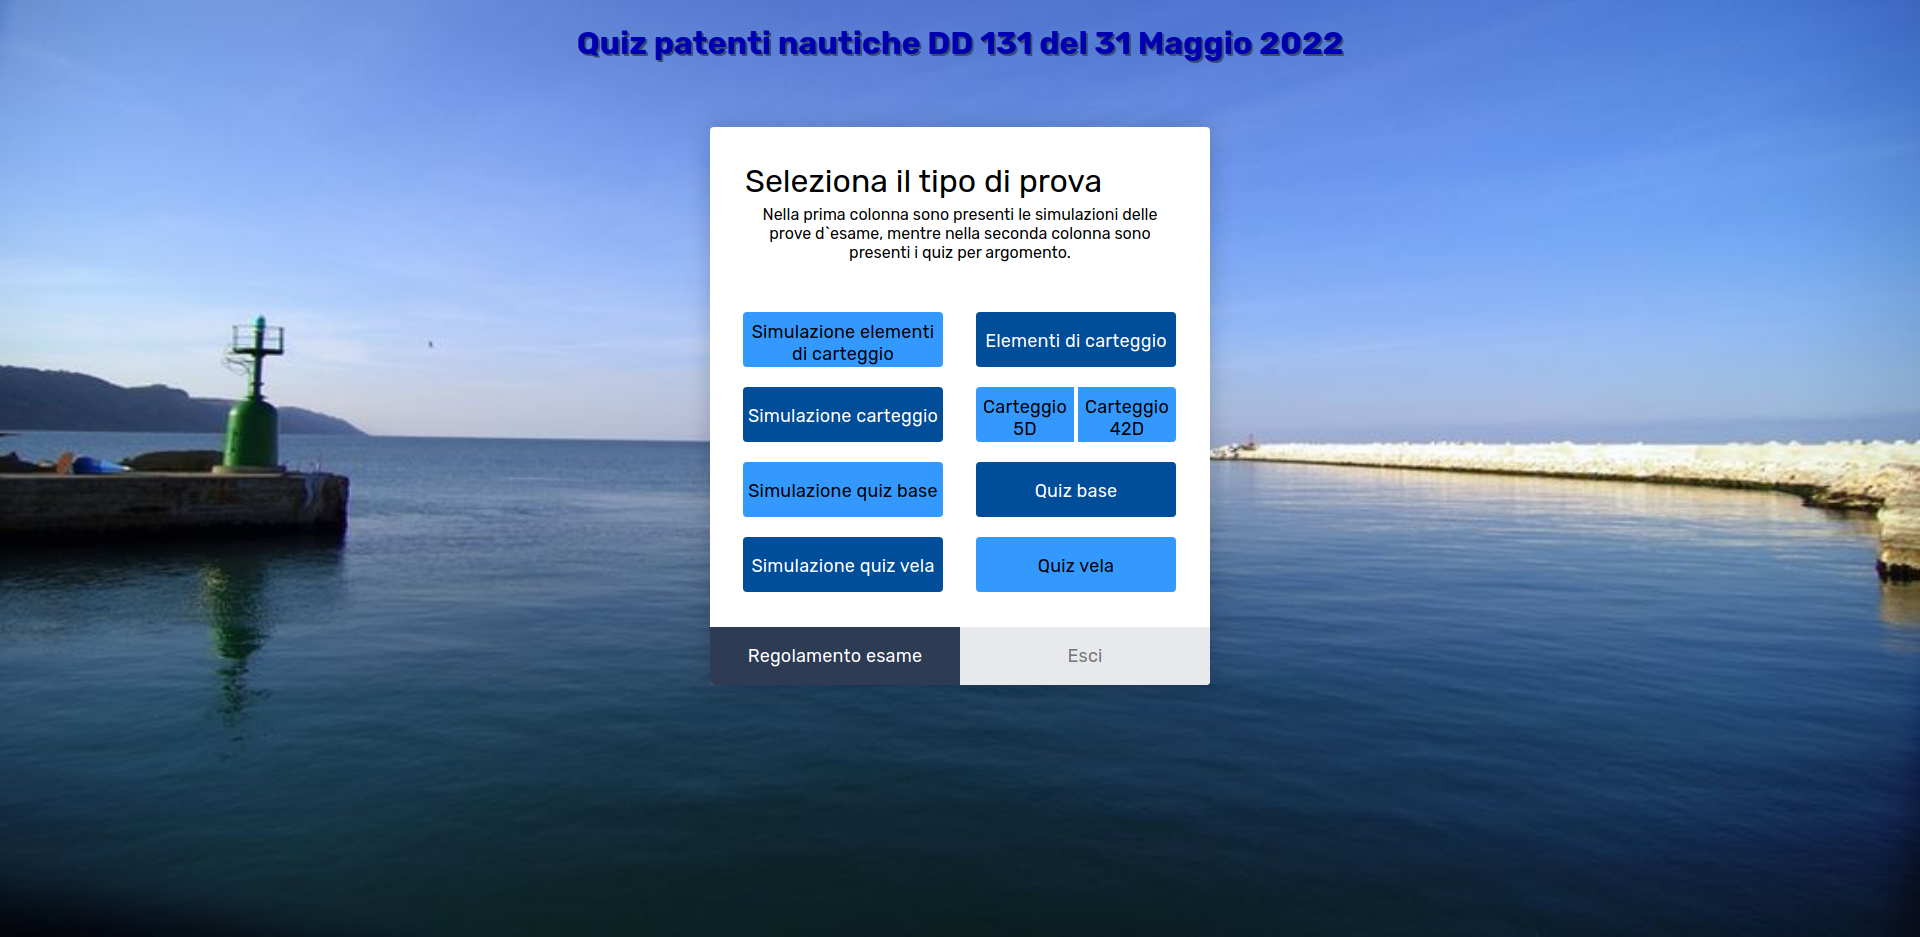
\includegraphics[scale=0.25]{Sites-images/07-Home_accesso_alle_prove.png}
		\caption{Pagina di selezione dei corsi.}
	\end{center}
\end{figure}

\textcolor{black}{Ora in ordine di rilevanza verranno presentati i file di ogni esercitazione, mettendo in evidenza le peculiarità di ognuno. I primi file saranno riportati maggiormente nella loro interezza in modo da esplicitare il metodo con il quale è stata condotta la costruzione dei restanti. Degli ultimi si riporteranno solo le parti salienti.}\\

\subsection{Presentazione delle pagine dei corsi}

\paragraph{\textcolor{black}{Simulazione elementi di carteggio}}\leavevmode\\

\begin{lstlisting}[language=php]
	if($_SESSION['permission'] !== "true"){
		/*control if user is logged*/
		if($_SESSION['mail'] !== null && $_SESSION['password'] !== null){
			
			$query = $utilities->getMysql()->query("SELECT password FROM user_table1 WHERE (email = '{$_SESSION['mail']}')");
			$tempArray = $query->fetch_array(MYSQLI_ASSOC);
			$password = $tempArray['password'];
			
			if($_SESSION['password'] !== $password){
				$_SESSION['user']     = "NotAllow";
				$_SESSION['mail']     = null;
				$_SESSION['password'] = null;
				header("Location: ../../main.php");
				exit;
			}
			/*in case of page reload*/
			$_SESSION['permission'] = "true";
			
		}else{
			$_SESSION['user']     = "NotAllow";
			$_SESSION['mail']     = null;
			$_SESSION['password'] = null;
			header("Location: ../../main.php");
			exit;
		}
	}
	
	/*find course properties*/
	$query = $utilities->getMysql()->query("SELECT * FROM charting_elements_properties WHERE (id = '1')");
	$tempArray = $query->fetch_array(MYSQLI_ASSOC);
	$maxQuestions = $tempArray['questions'];//<--- Very important field
	$maxErrors = $tempArray['errors'];//<--- Very important field
	
	/*find questions number*/
	$query = $utilities->getMysql()->query("SELECT COUNT(*) FROM charting_elements");
	$tempArray = $query->fetch_array(MYSQLI_ASSOC);
	$questionsNumber = $tempArray['COUNT(*)'];//<--- Very important field
	
	
	
	/*--------- GENERATE INDEXES AND EXTRACT QUESTIONS ----------*/
	
	$indexNumbers = array();
	$questions = array();
	
	$temp = 0;
	
	while($temp < $maxQuestions){
		
		if($_SESSION['numbers'][0] !== null){
			// if i'm here meaning that the page has been reloaded     
			if($indexNumbers[0] !== null){
				//generate number in recursive case
				$tempNum = random_int(1, $questionsNumber);
				//verify that the number isn't duplicated
				while(in_array($tempNum,$indexNumbers) || in_array($tempNum,$_SESSION['numbers'])){
					$tempNum = random_int(1, $questionsNumber);
				}
				
				//insert number
				$indexNumbers[$temp] = $tempNum; 
				
			}else{
				//generate number on base case
				$tempNum = random_int(1, $questionsNumber);
				//verify that the number is new (respect the past)
				while(in_array($tempNum,$_SESSION['numbers'])){
					$tempNum = random_int(1, $questionsNumber);
				}
				//insert number
				$indexNumbers[$temp] = $tempNum; 
			}
			
		}else{
			//if i'm here meaning that the page is new
			if($indexNumbers[0] !== null){
				//generate number in recursive case
				$tempNum = random_int(1, $questionsNumber);
				//verify that the number isn't duplicated
				while(in_array($tempNum,$indexNumbers)){
					$tempNum = random_int(1, $questionsNumber);
				}
				
				//insert number
				$indexNumbers[$temp] = $tempNum;
				
			}else{
				//generate number on base case
				$indexNumbers[$temp] = random_int(1, $questionsNumber);
			}
		}
		
		/*extract questions from db using the index generated*/
		$query = $utilities->getMysql()->query("SELECT * FROM charting_elements WHERE (id = '{$indexNumbers[$temp]}')");
		$tempArray = $query->fetch_array(MYSQLI_ASSOC);
		
		$questions[$temp] = array(
		"question_text"   => $tempArray['question_text'],
		"question1"       => $tempArray['question_1'],
		"question2"       => $tempArray['question_2'],
		"question3"       => $tempArray['question_3'],
		"question4"       => $tempArray['question_4'],
		"question5"       => $tempArray['question_5'],
		"answer1"         => $tempArray['answer_1'],
		"answer2"         => $tempArray['answer_2'],
		"answer3"         => $tempArray['answer_3'],
		"answer4"         => $tempArray['answer_4'],
		"answer5"         => $tempArray['answer_5'],
		);
		
		++$temp;
	}
	
	$_SESSION['numbers'] = $indexNumbers;
\end{lstlisting}

\textcolor{black}{Una delle prime operazioni che vengono svolte è il controllo dell'utente, per evitare l'accesso non autorizzato al servizio. Da notare inoltre che grazie alla variabile di sessione "permission" si garantisce che l'utente non venga espulso nel caso in cui ricarichi la pagina.\\
Successivamente si procede estraendo dal database le proprietà della simulazione, come il numero di domande da somministrare e il numero di errori massimi da poter commettere. Successivamente viene fatto il calcolo del numero delle domande presenti nel database in modo da poter stabilire il "range" per la selezione causale delle domande da presentare. Il fatto di contare ogni volta le domande presenti nel database garantisce che ogni nuova domanda inserita sia subito disponibile senza fare ulteriori aggiornamenti. Di conseguenza risulta semplificato il mantenimento e aggiornamento del database.\\
A questo punto si estraggono casualmente i vari indici delle domande da presentare. Questa operazione viene fatta con un ciclo "while" annidato che prosegue fino a che non siano stati generati senza ripetizioni (anche nei confronti dell'ultima esercitazione fatta) tutti gli indici richiesti. Per cercare di tenere alto il livello di efficienza delle operazioni l'ultima parte del ciclo "while" si compone della estrazione ed inserimento in un "array" delle domande permettendo di non dover svolgere un ulteriore ciclo.}\\
\bigskip
\textcolor{black}{Il codice "html" riportato inferiormente serve per mostrare come le informazioni estratte nella parte di "php" sono state integrate nella parte visibile della pagina. In generale si è usato il sistema "d'interrompere" il codice "html" richiamando il "tag" del "php" con l'ausilio comando "echo" per riportare le informazioni necessarie.}\\

\begin{lstlisting}[language=html]
	<!DOCTYPE html>
	<html lang="it" >
	<head>
	<meta charset="UTF-8">
	<title>Simulazione su elementi di carteggio nautico</title>
	<link rel='stylesheet' href='https://fonts.googleapis.com/css?family=Rubik:400,700'><link rel="stylesheet" href="simulationStyle.css">
	
	</head>
	<body>  
	
	<div class="welcomeText">
	<h1>Quiz patenti nautiche DD 131 del 31 Maggio 2022</h1>
	<h2>Simulazione sulle domande su elementi di carteggio nautico</h2>
	</div>
	
	<div class="question-form">
	<form method="post">
	<h1><?php
	if($indexNumbers[1] !== null){
		echo "Indice domande: ";
		$temp = 0;
		
		while($temp < $maxQuestions){
			echo $indexNumbers[$temp]." ";
			++$temp;
		}
		
	}else{
		echo "Indice domanda: ".$indexNumbers[0];
	}
	?>
	</h1>
	<div class="content">
	<?php 
	$temp = 0;
	while($temp < $maxQuestions){
		echo "<b>".$questions[$temp]["question_text"]."</b><br>";
		echo"<br>";
		echo $questions[$temp]["question1"]."<br>";
		echo $questions[$temp]["question2"]."<br>";
		echo $questions[$temp]["question3"]."<br>";
		echo $questions[$temp]["question4"]."<br>";
		echo $questions[$temp]["question5"]."<br>";
		echo"<br>";
		++$temp;
	}
	?> 
	</div>
	<div class="actions">
	<input type="button" name="revision" value="Guarda la soluzione" id="revision" onclick="check()"/>
	<div id="chart">Non hai la carta nautica? <a href="../Nautical_Charts/Carta_Nautica_5D.pdf" download> Scaricala qui</a></div>
	</div>
	<div id="answer">
	<?php
	$temp = 0;
	while($temp < $maxQuestions){
		if($indexNumbers[1] !== null){
			$tempNumber = $temp + 1;
			echo"<h3>Soluzione domanda: ".$tempNumber." </h3><br>"; 
		}
		echo"Soluzione quesito 1: <b>".$questions[$temp]["answer1"]."</b><br>";
		echo"Soluzione quesito 2: <b>".$questions[$temp]["answer2"]."</b><br>";
		echo"Soluzione quesito 3: <b>".$questions[$temp]["answer3"]."</b><br>";
		echo"Soluzione quesito 4: <b>".$questions[$temp]["answer4"]."</b><br>";
		echo"Soluzione quesito 5: <b>".$questions[$temp]["answer5"]."</b><br>";
		echo"<br>";
		++$temp;
	}
	?>
	<h3><?php
	if($maxErrors > 1){
		echo "La prova e' stata superata se si sono commessi massimo ".$maxErrors." errori.";
	}else{
		echo "La prova e' stata superata se e' stato commesso massimo ".$maxErrors." errore.";  
	}
	
	?></h3>
	</div>
	<div class="foot">
	<input type="submit" name="cancel" value="Esci dalla simulazione" id="button2"/>
	<input type="button" name="nextPage" value="Prova successiva" id="button1" onclick="next()"/>
	</div>
	</form>
	</div>
\end{lstlisting}

\textcolor{black}{Un problema che si solleva a questo punto dello sviluppo è la creazione di un sistema che permetta di nascondere la risposta del quesito, permettendo quindi l'esercizio. Questa cosa è realizzabile solo con il "javascript" che permette lato "front-end" di animare le varie parti del "html".\\
Si riportata lo "script" che è stato scritto per risolvere il problema.}\\

\begin{lstlisting}[language=java]
	<script>
	
	/*hide elements at the beginning*/
	var x = document.getElementById("answer");
	x.style.display = "none";
	
	/*show elements when the button is clicked*/
	function check(){
		var x = document.getElementById("answer");
		
		if(x.style.display === "none"){
			x.style.display = "block";
		}else{
			x.style.display = "none";
		}	
	}
	
	function next(){
		location.reload();  
	}
	</script>
\end{lstlisting}

\textcolor{black}{La funzione "check" viene evocata dal pulsante identificato come "revision" e permette di mostrare o di nascondere la parte in "html" contrassegnata come "answer" (inizialmente nascosta).\\
Siccome ogni esercitazione viene organizzata nella parte di codice in "php", eseguita soltanto durante il caricamento della pagina, come ultima cosa è stata dichiarata una funzione invocata dal pulsante "nextPage" per forzare il "reloading" della pagina, generando di fatto (nelle modalità vista prima) una nuova esercitazione.}\\
\bigskip
\textcolor{black}{Finito di presentare il codice della simulazione, si desidera procedere con quello dell'esercitazione riferita sempre allo stesso tipo di domande. Incominciando ad analizzare il codice in "php"}.

\begin{figure}[h]
	\begin{center}
		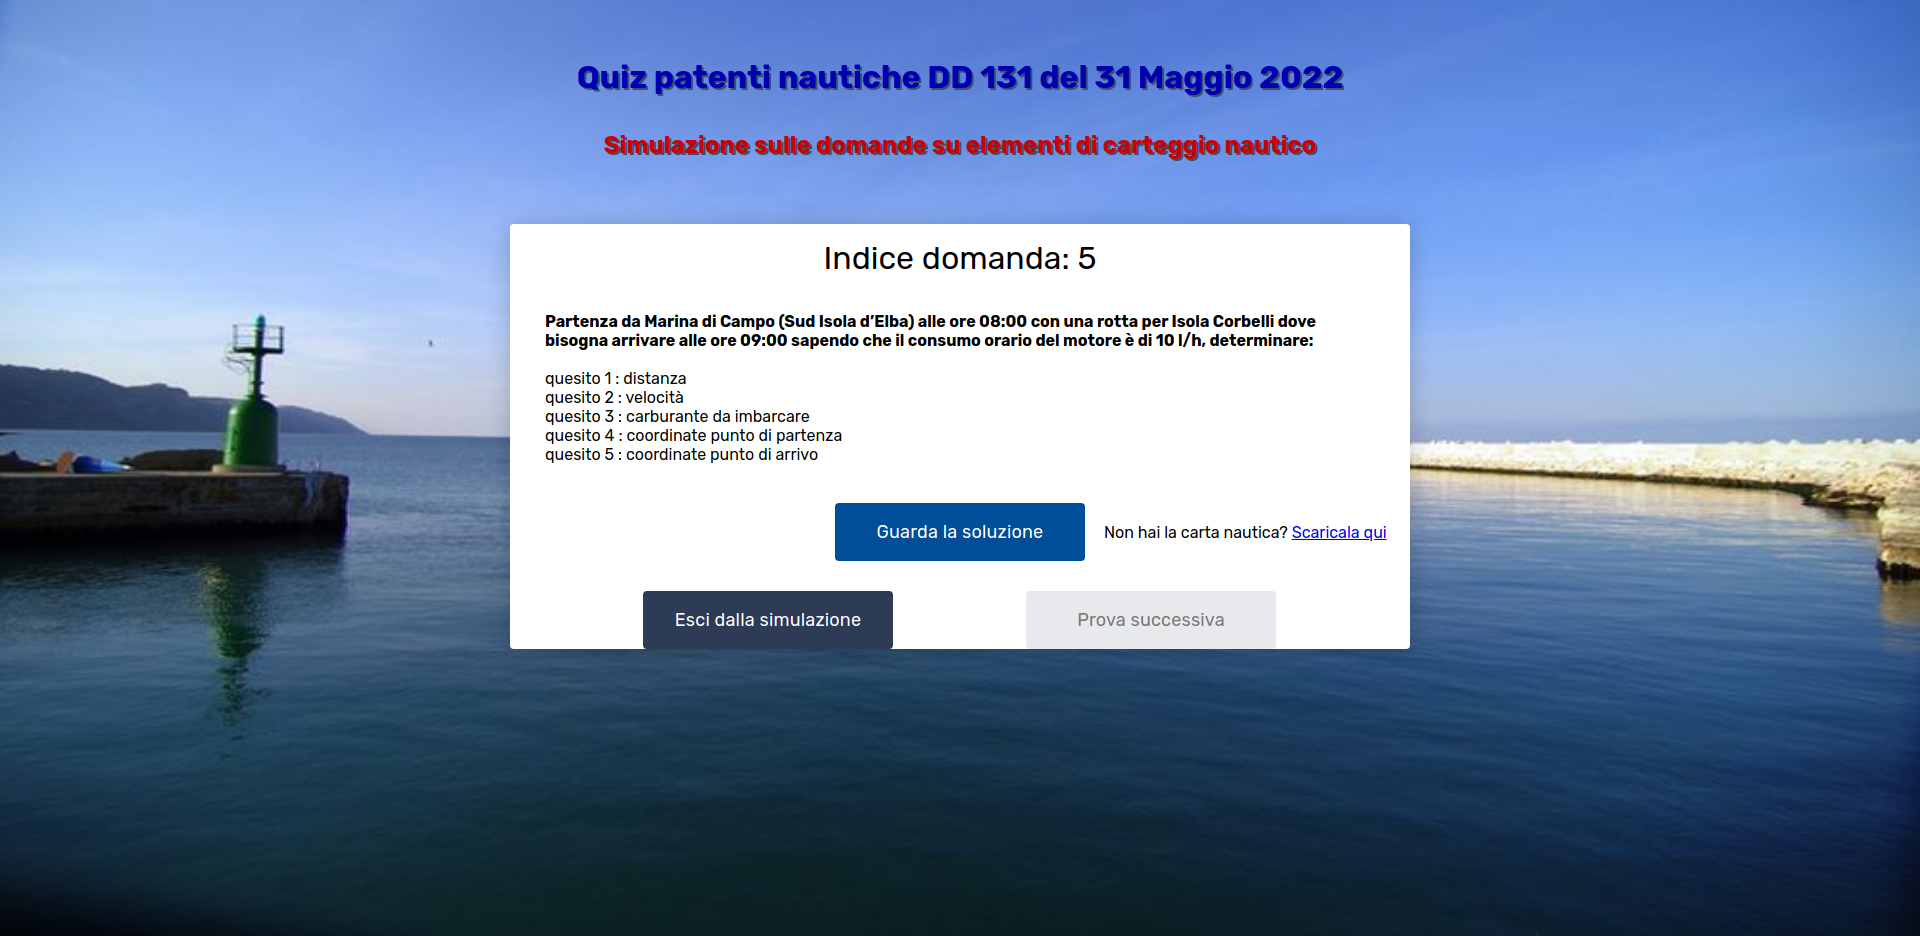
\includegraphics[scale=0.25]{Sites-images/12-Simulazione_elementi_di_carteggio.png}
		\caption{Pagina della simulazione elementi di carteggio.}
	\end{center}
\end{figure}

\begin{figure}[h]
	\begin{center}
		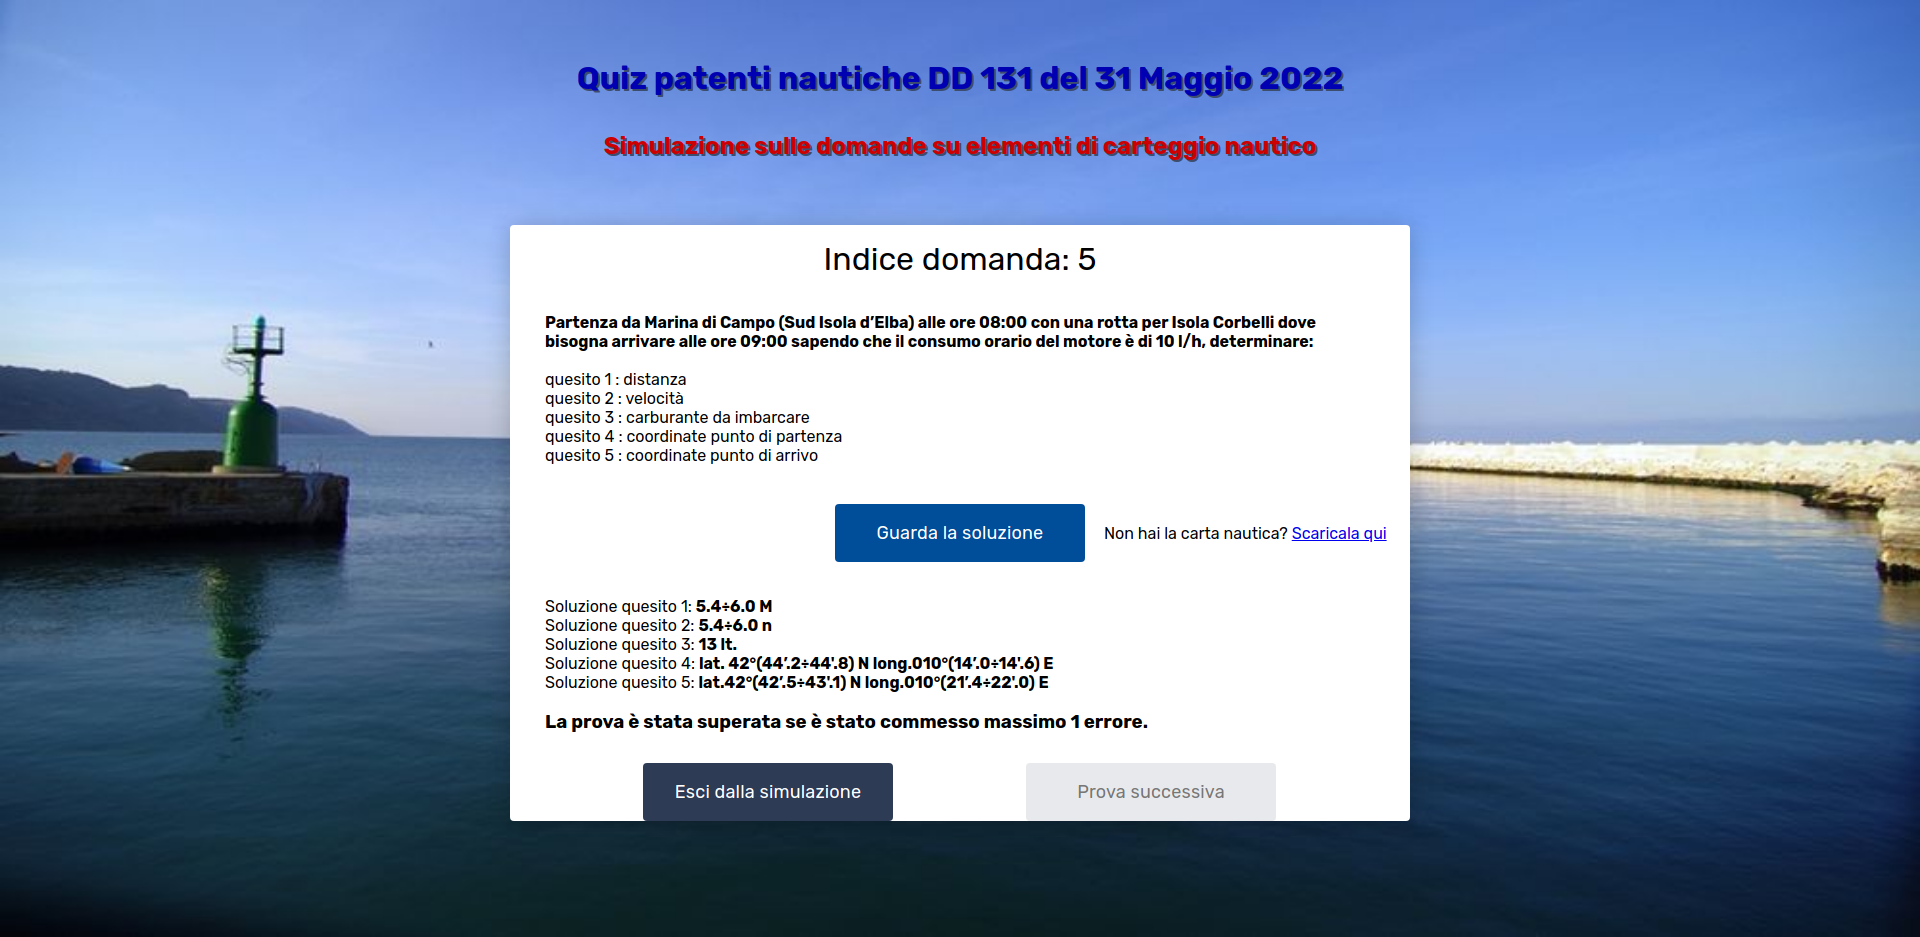
\includegraphics[scale=0.25]{Sites-images/13-Simulazione_elementi_di_carteggio-con_soluzioni.png}
		\caption{Pagina della simulazione elementi di carteggio con le soluzioni.}
	\end{center}
\end{figure}

\paragraph{\textcolor{black}{Elementi di carteggio (esercitazione)}}\leavevmode\\

\begin{lstlisting}[language=php]
	
	if($_SESSION['permission'] !== "true"){
		/*control if user is logged*/
		if($_SESSION['mail'] !== null && $_SESSION['password'] !== null){
			
			$query = $utilities->getMysql()->query("SELECT password FROM user_table1 WHERE (email = '{$_SESSION['mail']}')");
			$tempArray = $query->fetch_array(MYSQLI_ASSOC);
			$password = $tempArray['password'];
			
			if($_SESSION['password'] !== $password){
				$_SESSION['user']     = "NotAllow";
				$_SESSION['mail']     = null;
				$_SESSION['password'] = null;
				header("Location: ../../main.php");
				exit;
			}
			/*in case of page reload*/
			$_SESSION['permission'] = "true";
			
		}else{
			$_SESSION['user']     = "NotAllow";
			$_SESSION['mail']     = null;
			$_SESSION['password'] = null;
			header("Location: ../../main.php");
			exit;
		}
	}
	
	/*---------- END USER VERIFY ----------*/
	
	/*set count variable*/
	if($_SESSION['numbers'] == null){
		$_SESSION['numbers'] = 1;
	}
	
	
	/*find questions number*/
	$query = $utilities->getMysql()->query("SELECT COUNT(*) FROM charting_elements");
	$tempArray = $query->fetch_array(MYSQLI_ASSOC);
	$maxQuestions = $tempArray['COUNT(*)'];//<--- Very important field
	
	
	/*---------- START BUTTONS PART ----------*/
	
	if(isset($_POST['prevPage'])){
		if($_SESSION['numbers'] - 1 >= 1 && $_SESSION['numbers'] !== null){
			--$_SESSION['numbers'];
		}else{
			$utilities->Popup("Non e' possibile visualizzare la domanda precedente");
		}
	}
	
	if(isset($_POST['cancel'])){
		$_SESSION['permission'] = null;
		$_SESSION['numbers']     = null;
		header("Location: ../entry.php");
		exit;
	}
	
	if(isset($_POST['nextPage'])){
		if($_SESSION['numbers'] + 1 <= $maxQuestions && $_SESSION['numbers'] !== null){
			++$_SESSION['numbers'];
		}else{
			$utilities->Popup("Non e' possibile visualizzare la domanda successiva");
		}
	}
	
	/*---------- GENERATE QUESTIONS ----------*/
	
	$query = $utilities->getMysql()->query("SELECT * FROM charting_elements WHERE (id = '{$_SESSION['numbers']}')");
	$tempArray = $query->fetch_array(MYSQLI_ASSOC);
	$question_text = $tempArray['question_text'];
	$question1     = $tempArray['question_1'];
	$question2     = $tempArray['question_2'];
	$question3     = $tempArray['question_3'];
	$question4     = $tempArray['question_4'];
	$question5     = $tempArray['question_5'];
	$answer1       = $tempArray['answer_1'];
	$answer2       = $tempArray['answer_2'];
	$answer3       = $tempArray['answer_3'];
	$answer4       = $tempArray['answer_4'];
	$answer5       = $tempArray['answer_5'];
\end{lstlisting}

\textcolor{black}{Anche in questo caso la prima cosa che viene fatta è sempre il controllo dell'utente (da questo punto non più riportato nelle parti di codice successive).  Durante la generazione di una nuova esercitazione viene scritta una variabile di sessione con l'indice della domanda corrente, in modo che dopo il "reload" si possa accedere alla domanda successiva o alla precedente se è possibile (cioè a meno di non trovarsi agli estremi della lista di domande). Durante il primo accesso all'esercitazione la varaibile viene sempre instanziata con il valore di 1, siccome per specifica le domande sono conteggiate a partire dal numero 1 e non dallo 0 come abitudine informatica.\\
Saltata la parte che riguarda la gestione dei pulsantisi mostra come in questo caso, non dovendo gestire più di una domanda per volta,  si sia preferito dichiarare tante variabili quante le informazioni necessarie, al posto di dichiarare un "array" come nel caso precedente.\\
Lampante a questo punto sarà la semplicità con la quale le informazioni sono state riportate nella parte visibile della pagina. Dato che non è stato mostrato prima il codice "html" tipico delle esercitazioni, anche in questo caso viene riportato nella sua interezza, per dar modo di comprendere questo aspetto.}\\

\begin{lstlisting}[language=html]
	<html lang="it" >
	<head>
	<meta charset="UTF-8">
	<title>Esercitazione su elementi di carteggio nautico</title>
	<link rel='stylesheet' href='https://fonts.googleapis.com/css?family=Rubik:400,700'><link rel="stylesheet" href="exerciseStyle.css">
	
	</head>
	<body>  
	
	<div class="welcomeText">
	<h1>Quiz patenti nautiche DD 131 del 31 Maggio 2022</h1>
	<h2>Esercitazione sulle domande su elementi di carteggio nautico</h2>
	</div>
	
	<div class="question-form">
	<form method="post">
	<h1><?php
	echo "Indice domanda: ".$_SESSION['numbers']." / ". $maxQuestions;
	?>
	</h1>
	<div class="content">
	<?php 
	echo "<b>".$question_text."</b><br>";
	echo"<br>";
	echo $question1."<br>";
	echo $question2."<br>";
	echo $question3."<br>";
	echo $question4."<br>";
	echo $question5;
	?> 
	</div>
	<div class="actions">
	<input type="button" name="revision" value="Guarda la soluzione" id="revision" onclick="check()"/>
	<div id="chart">Non hai la carta nautica? <a href="../Nautical_Charts/Carta_Nautica_5D.pdf" download> Scaricala qui</a></div>
	</div>
	<div id="answer">
	<?php
	echo "Soluzione quesito 1: <b>".$answer1."</b><br>";
	echo "Soluzione quesito 2: <b>".$answer2."</b><br>";
	echo "Soluzione quesito 3: <b>".$answer3."</b><br>";
	echo "Soluzione quesito 4: <b>".$answer4."</b><br>";
	echo "Soluzione quesito 5: <b>".$answer5."</b>";
	?>
	</div>
	<div class="foot">
	<input type="submit" name="prevPage" value="Domanda precedente" id="button3"/>
	<input type="submit" name="cancel" value="Esci dalla esercitazione" id="button2"/>
	<input type="submit" name="nextPage" value="Domanda successiva" id="button1"/>
	</div>
	</form>
	</div>
\end{lstlisting}

\textcolor{black}{La parte di "scripting" non viene riportata poiché simile a quella precedente.}\\
\bigskip
\textcolor{black}{Si analizzano ora le peculiarità della prova di carteggio.}\\

\begin{figure}[h]
	\begin{center}
		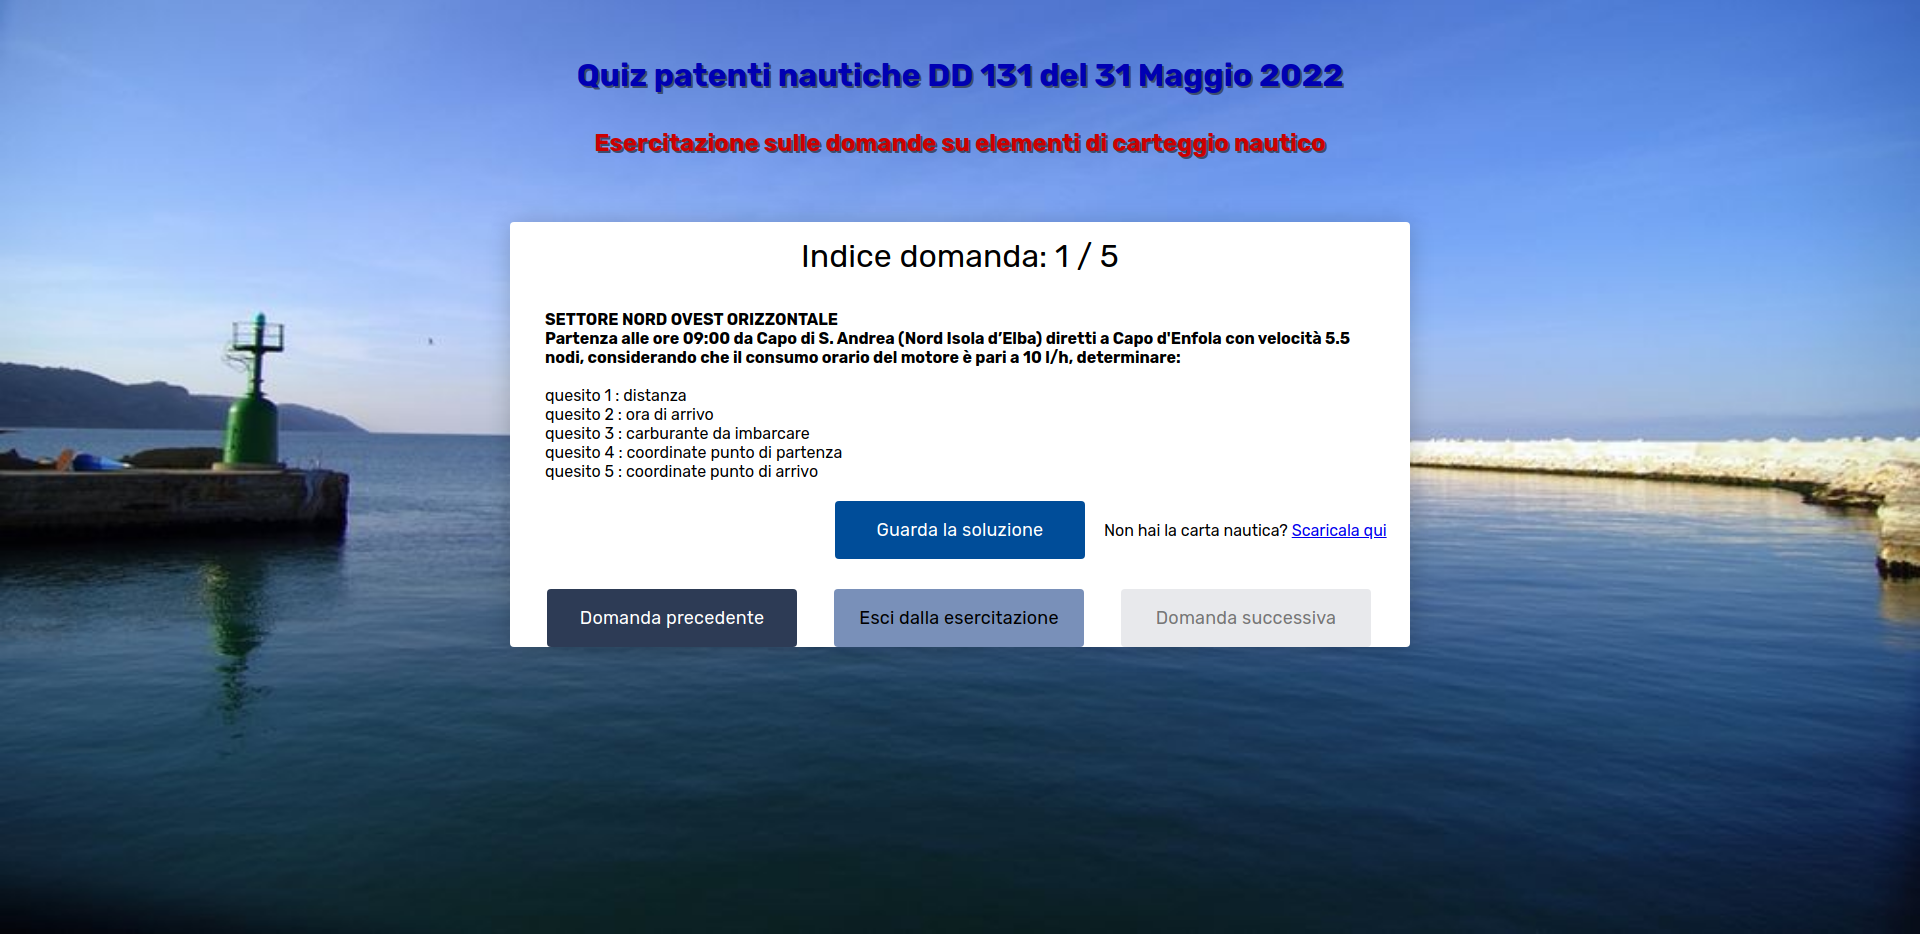
\includegraphics[scale=0.25]{Sites-images/14-Elementi_di_carteggio.png}
		\caption{Pagina degli elementi di carteggio.}
	\end{center}
\end{figure}

\begin{figure}[h]
	\begin{center}
		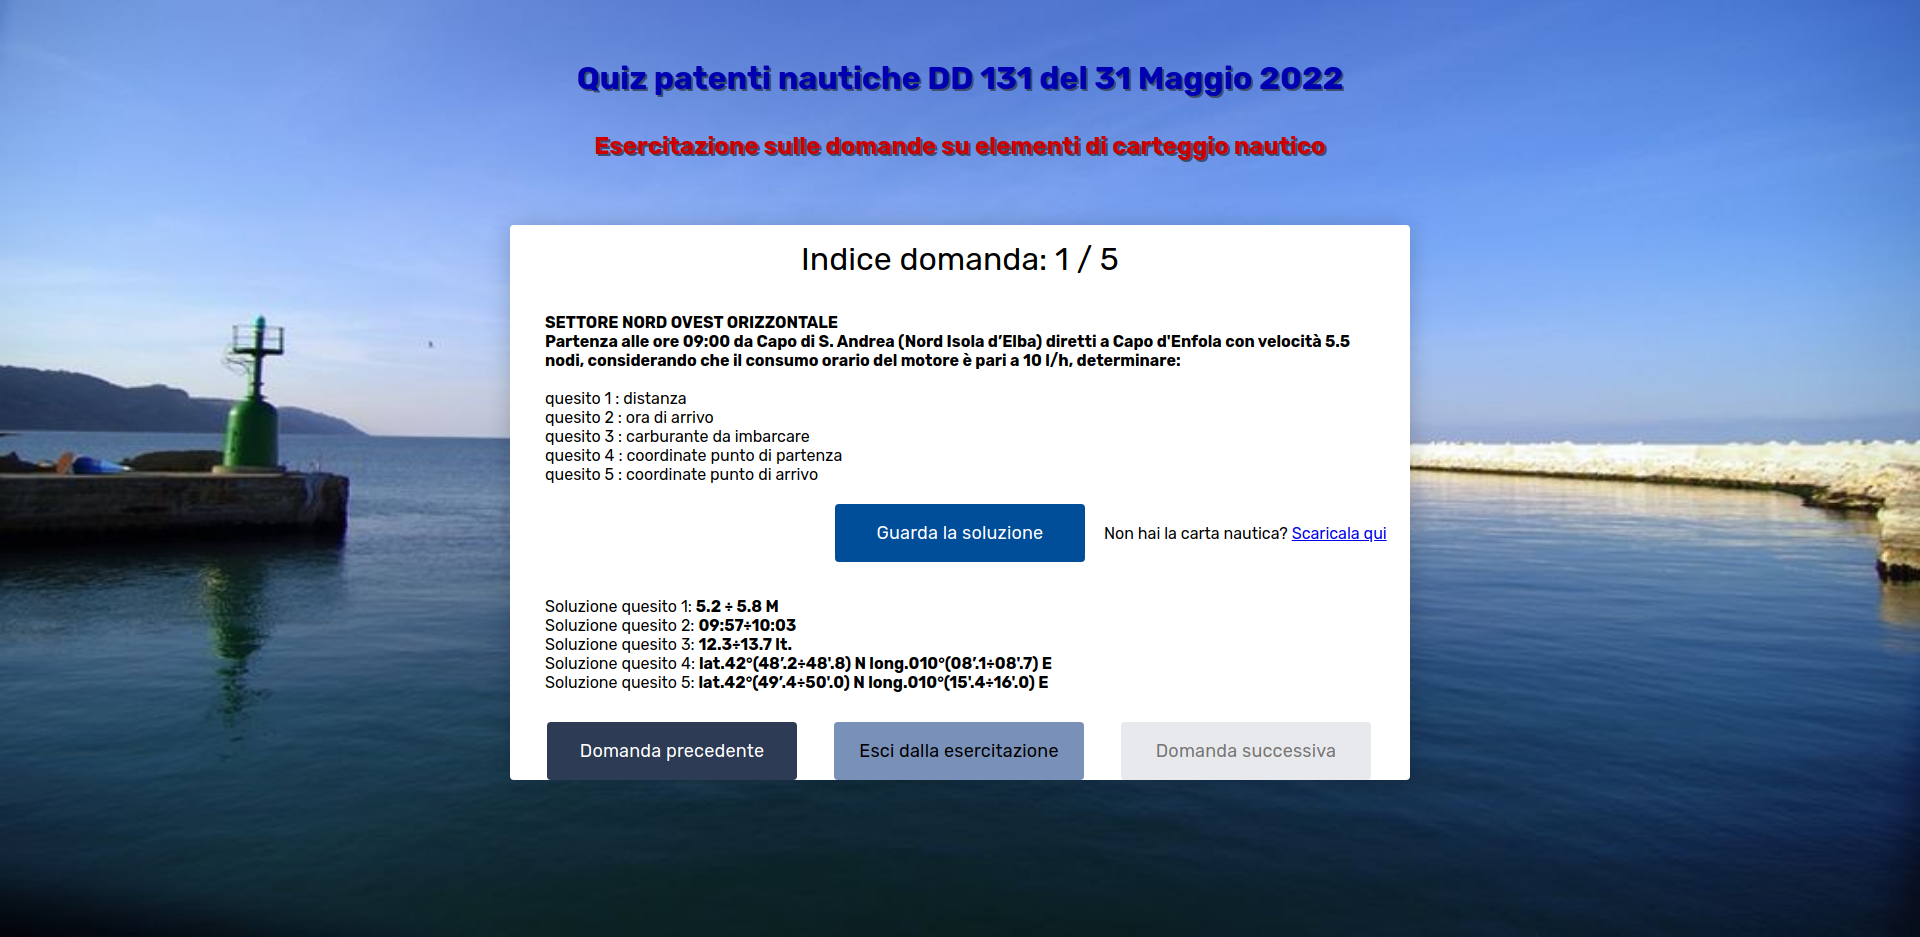
\includegraphics[scale=0.25]{Sites-images/15-Elementi_di_carteggio-con_soluzioni.png}
		\caption{Pagina degli elementi di carteggio con soluzioni.}
	\end{center}
\end{figure}

\paragraph{\textcolor{black}{Simulazione carteggio}}\leavevmode\\

\textcolor{black}{La cosa che è d'interesse in questo caso è la gestione e presentazione di domande prese da due insiemi differenti, ovvero, quelle sulla carta nautica "5D" e "42D".}\\ 

\begin{lstlisting}[language=php]
	/*find course properties*/
	$query = $utilities->getMysql()->query("SELECT * FROM charting_test_properties WHERE (id = '1')");
	$tempArray = $query->fetch_array(MYSQLI_ASSOC);
	
	$max5DQuestions = $tempArray['5d_questions'];//<--- Very important field
	$max42DQuestions = $tempArray['42d_questions'];//<--- Very important field
	$maxErrors = $tempArray['errors'];//<--- Very important field
	
	/*find current questions numbers*/
	$query = $utilities->getMysql()->query("SELECT COUNT(*) FROM charting_test_5d");
	$tempArray = $query->fetch_array(MYSQLI_ASSOC);
	$questionsNumber5D = $tempArray['COUNT(*)'];//<--- Very important field
	
	$query = $utilities->getMysql()->query("SELECT COUNT(*) FROM charting_test_42d");
	$tempArray = $query->fetch_array(MYSQLI_ASSOC);
	$questionsNumber42D = $tempArray['COUNT(*)'];//<--- Very important field
	
	
	/*--------- GENERATE THE INDEXES AND extract questions---------*/
	$questionsIndex = 0;
	$indexNumbers = array();
	$questions = array();
	
	//---------- CHART 5D
	$temp = 0;
	while($temp < $max5DQuestions){
		
		if($_SESSION['numbers']['5d'][0] !== null){
			// if i'm here meaning that the page has been reloaded      
			if($indexNumbers['5d'][0] !== null){
				//generate number in recursive case
				$tempNum = random_int(1, $questionsNumber5D); // this 1 is because i know that the questions starts form 1 into db
				//verify that number isn't duplicated
				while(in_array($tempNum,$indexNumbers['5d']) || in_array($tempNum,$_SESSION['numbers']['5d'])){
					$tempNum = random_int(1, $questionsNumber5D);
				}
				
				//insert number
				$indexNumbers['5d'][$temp] = $tempNum; 
				
			}else{
				//generate number on base case
				$tempNum = random_int(1, $questionsNumber5D);
				//verify that the number is new (respect the past)
				while(in_array($tempNum,$_SESSION['numbers']['5d'])){
					$tempNum = random_int(1, $questionsNumber5D);
				}
				//insert number
				$indexNumbers['5d'][$temp] = $tempNum; 
			}
			
		}else{
			
			//if i'm here meaning that the page is new
			if($indexNumbers['5d'][0] !== null){
				//generate number in recursive case
				$tempNum = random_int(1, $questionsNumber5D);
				//verify that the number isn't duplicated
				while(in_array($tempNum,$indexNumbers['5d'])){
					$tempNum = random_int(1, $questionsNumber5D);
				}
				
				//insert number
				$indexNumbers['5d'][$temp] = $tempNum;
				
			}else{
				//generate number on base case
				$indexNumbers['5d'][$temp] = random_int(1, $questionsNumber5D);
			}
		}
		
		//extract questions from db
		$query = $utilities->getMysql()->query("SELECT * FROM charting_test_5d WHERE (id = '{$indexNumbers['5d'][$temp]}')");
		$tempArray = $query->fetch_array(MYSQLI_ASSOC);  
		
		$questions[$questionsIndex] = array(
		"index"         => $tempArray['id'],
		"question_text" => $tempArray['question_text'],
		"answer"        => $tempArray['answer'],
		"area"		=> $tempArray['area'],
		"is42d"         => false,
		);
		++$questionsIndex;
		
		++$temp;
	}
	
	//---------- CHART 42D
	$temp = 0;
	while($temp < $max42DQuestions){
		
		if($_SESSION['numbers']['42d'][0] !== null){
			// if i'm here meaning that the page has been reloaded     
			if($indexNumbers['42d'][0] !== null){
				//generate number in recursive case
				$tempNum = random_int(1, $questionsNumber42D); // this 1 is because i know that the questions starts form 1 into db
				//verify that the number isn't duplicated
				while(in_array($tempNum,$indexNumbers['42d']) || in_array($tempNum,$_SESSION['numbers']['42d'])){
					$tempNum = random_int(1, $questionsNumber42D);
				}
				
				//insert number
				$indexNumbers['42d'][$temp] = $tempNum; 
				
			}else{
				//generate number on base case
				$tempNum = random_int(1, $questionsNumber42D);
				//verify that the number is new (respect the past)
				while(in_array($tempNum,$_SESSION['numbers']['42d'])){
					$tempNum = random_int(1, $questionsNumber42D);
				}
				//insert number
				$indexNumbers['42d'][$temp] = $tempNum; 
			}
			
		}else{
			//if i'm here meaning that the page is new
			if($indexNumbers['42d'][0] !== null){
				//generate number in recursive case
				$tempNum = random_int(1, $questionsNumber42D);
				//verify that the number isn't duplicated
				while(in_array($tempNum,$indexNumbers['42d'])){
					$tempNum = random_int(1, $questionsNumber42D);
				}
				
				//insert number
				$indexNumbers['42d'][$temp] = $tempNum;
				
			}else{
				//generate number on base case
				$indexNumbers['42d'][$temp] = random_int(1, $questionsNumber42D);
			}
		}
		
		//extract questions from db
		$query = $utilities->getMysql()->query("SELECT * FROM charting_test_42d WHERE (id = '{$indexNumbers['42d'][$temp]}')");
		$tempArray = $query->fetch_array(MYSQLI_ASSOC);  
		
		$questions[$questionsIndex] = array(
		"index"         => $tempArray['id'],
		"question_text" => $tempArray['question_text'],
		"answer"        => $tempArray['answer'],
		"area"		=> $tempArray['area'],	
		"is42d"         => true,
		);
		++$questionsIndex;
		
		++$temp;
	}
	
	
	$_SESSION['numbers'] = $indexNumbers;
	
	$totalQuestions = count($questions);
\end{lstlisting}
\textcolor{black}{In generale l'estrazione delle domande non avviene in modi differenti rispetto a quanto presentato in passato. Si può osservare che per ogni tipo di domande è stato fatto un ciclo "while" con la stessa logica del precedente. In questo caso la scelta di un doppio ciclo (uno per ogni insieme di domande) potrebbe non risultare tra le più efficienti in assoluto, ma aumenta la semplicità del codice, permettendo di vedere il problema del reperimento delle informazioni come diviso in due parti. Però si è comunque cercato di rendere il codice efficiente usando un solo "array" (al posto di due come si sarebbe portati a pensare) per memorizzare tutte le domande estratte, in modo da risparmiare spazio in memoria. Il campo "is42d" permette di distinguere tra i due tipi di domande.\\
Il resto del codice della pagina non presenta ulteriori diversità.}\\

\begin{figure}[h]
	\begin{center}
		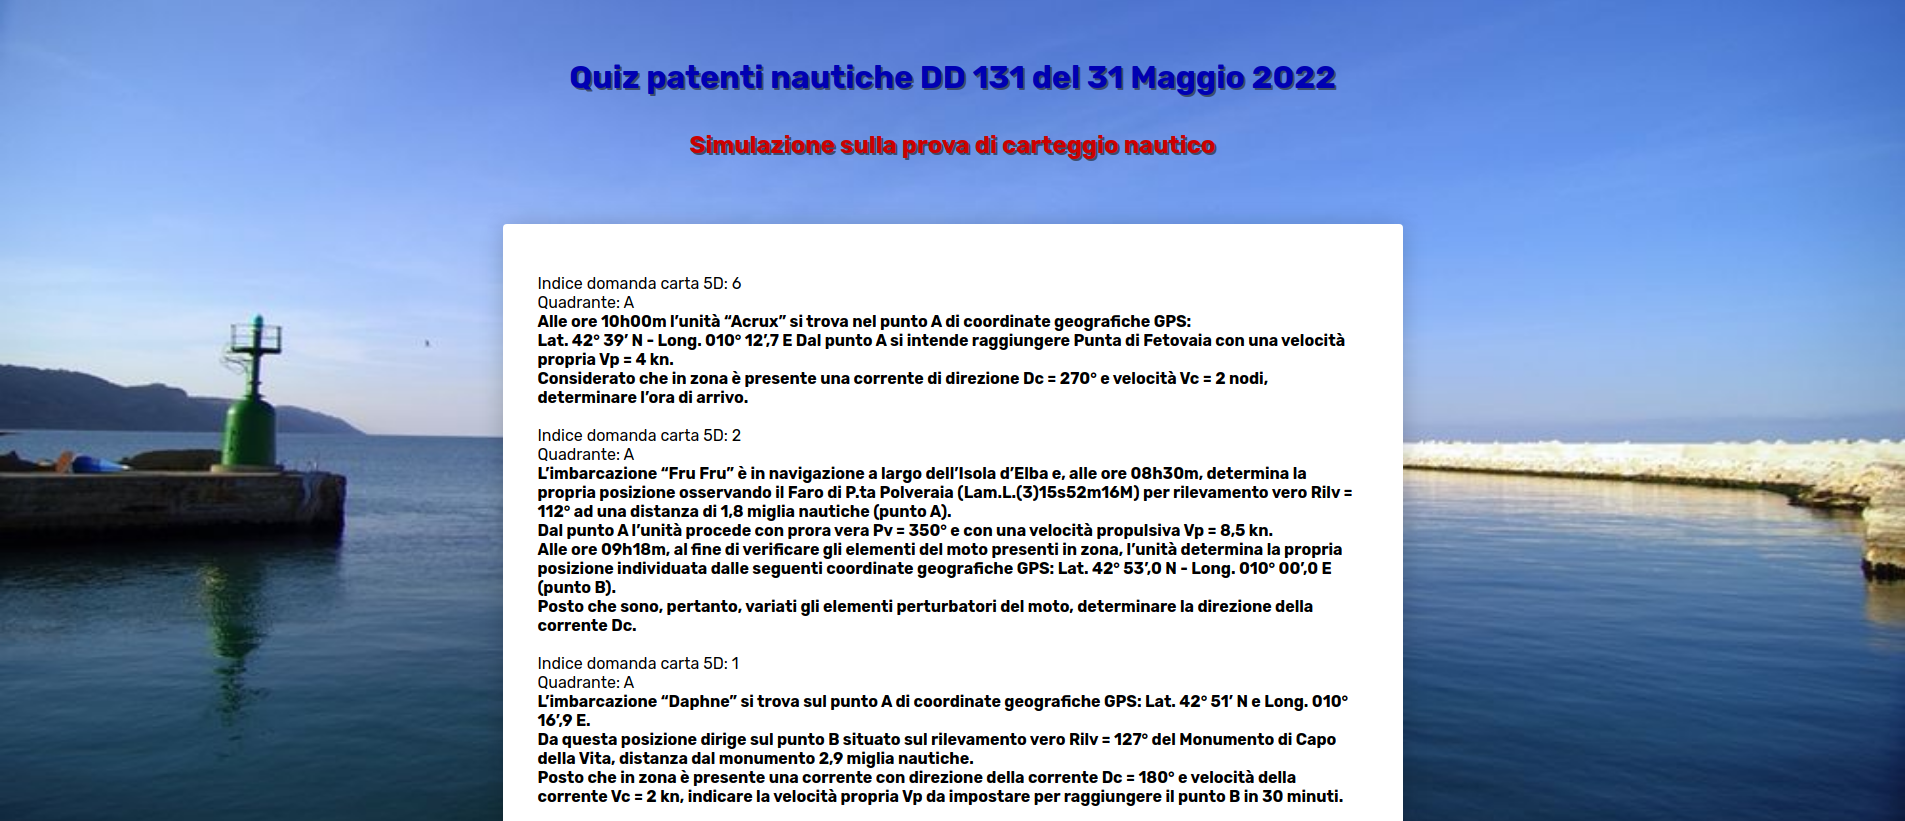
\includegraphics[scale=0.25]{Sites-images/16-Simulazione_carteggio1.png}
			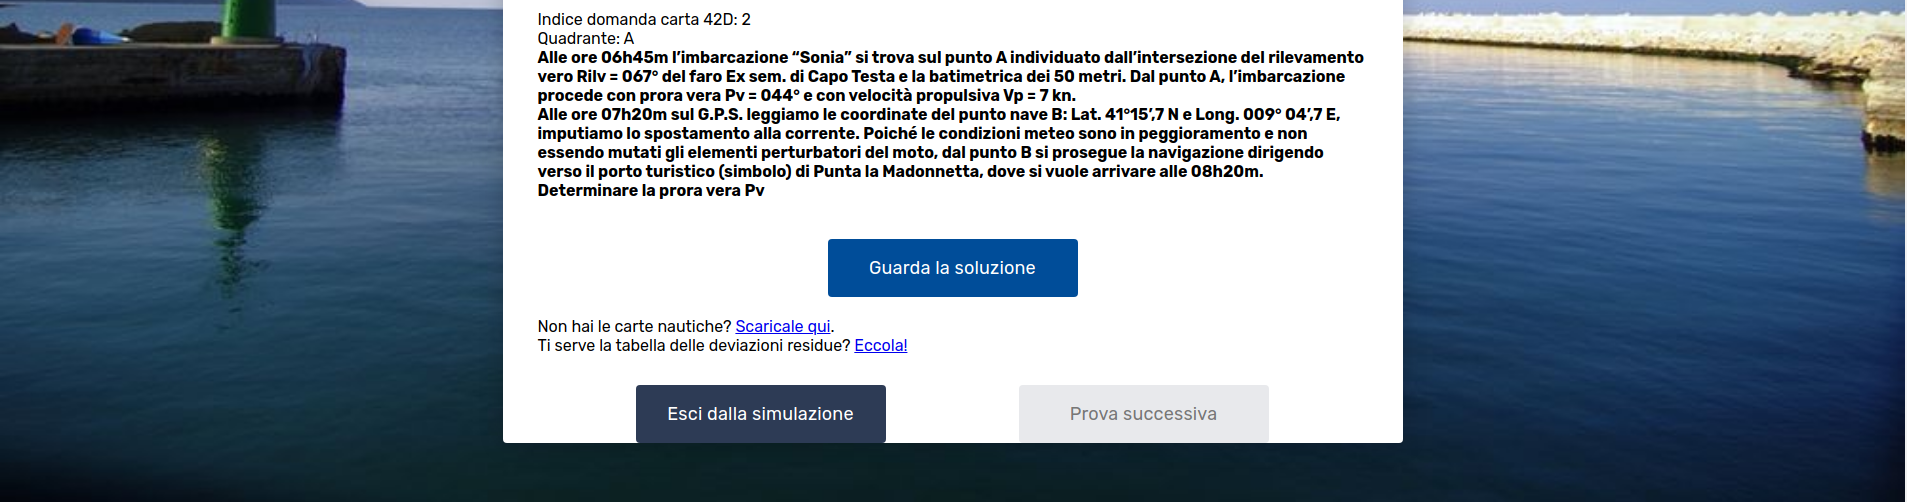
\includegraphics[scale=0.25]{Sites-images/17-Simulazione_carteggio2.png}
		\caption{Pagina di simulazione del carteggio.}
		(Ricomposta)
	\end{center}
\end{figure}

\begin{figure}[h]
	\begin{center}
		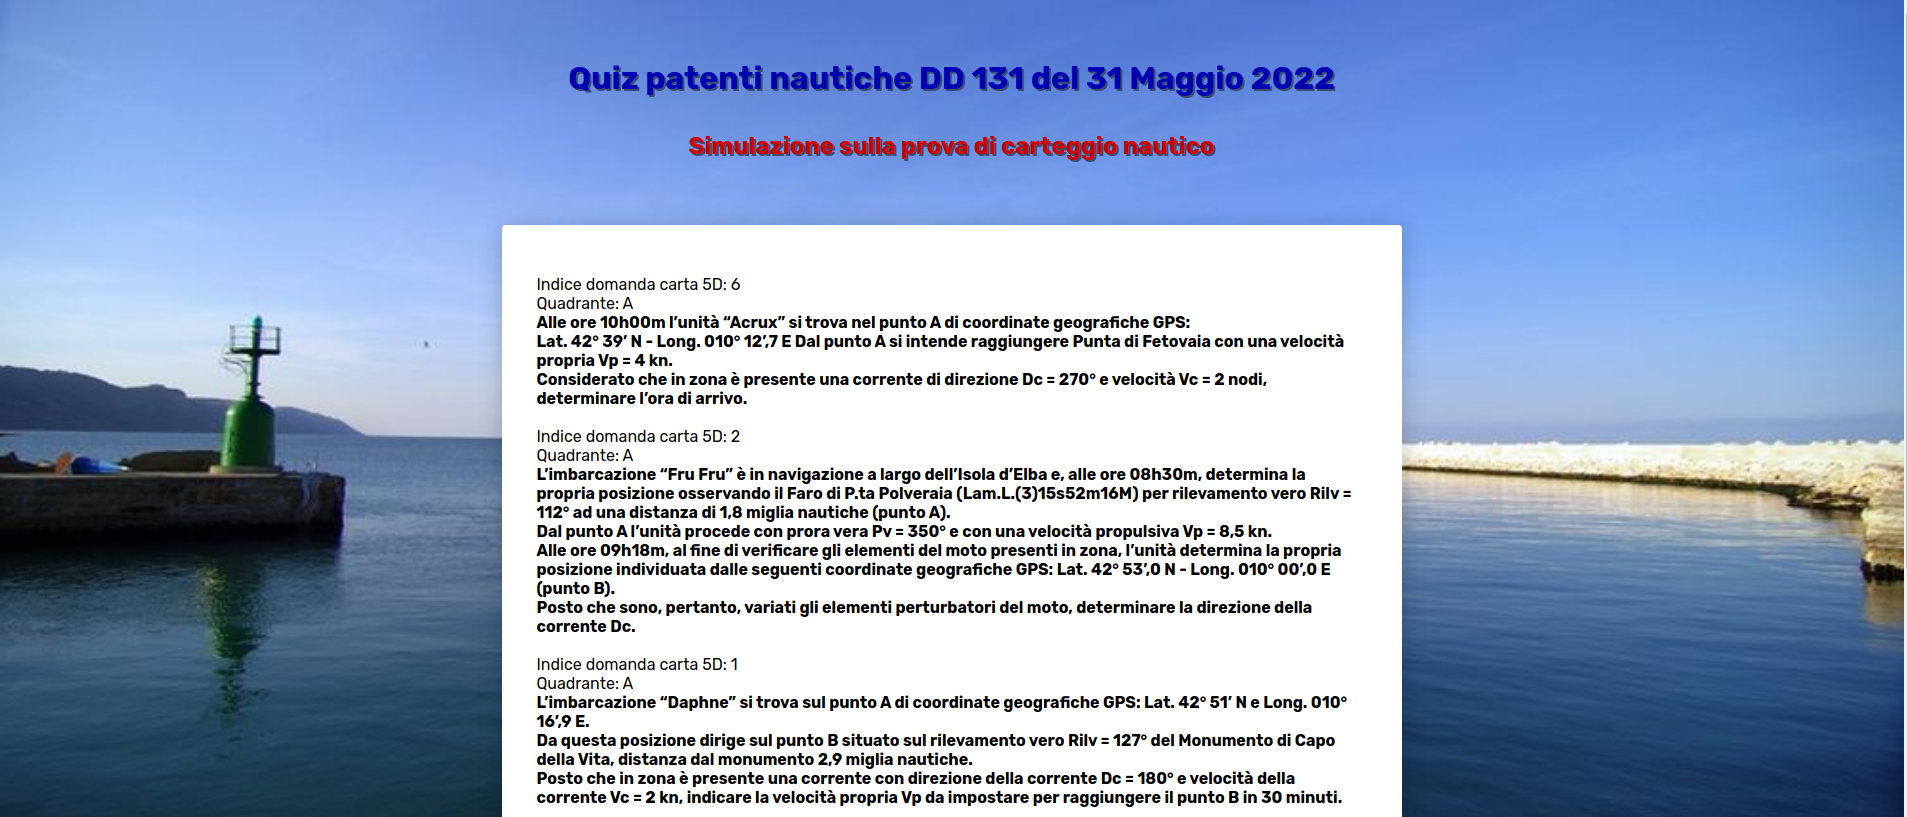
\includegraphics[scale=0.25]{Sites-images/18-Simulazione_carteggio-con_soluzioni1.png}
		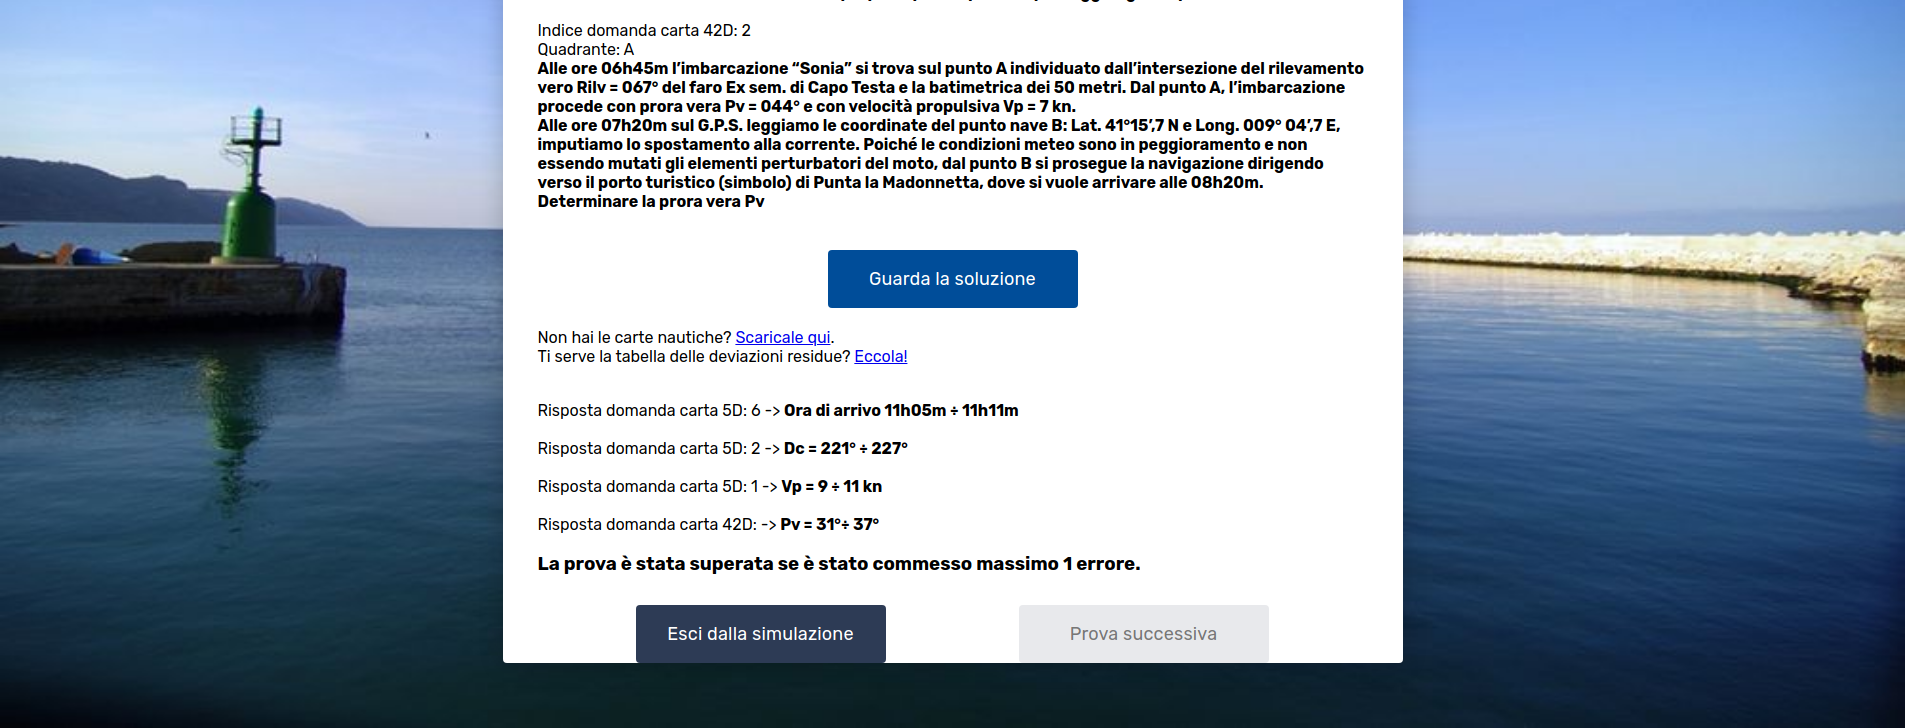
\includegraphics[scale=0.25]{Sites-images/19-Simulazione_carteggio-con_soluzioni2.png}
		\caption{Pagina di simulazione del carteggio con soluzioni.}
		(Ricomposta)
	\end{center}
\end{figure}

\paragraph{\textcolor{black}{Carteggio 5D e 42D (esercitazione)}}\leavevmode\\
\textcolor{black}{Durante la spiegazione di questa parte, sono state accorpate le due pagine distinte per l'esercitazione nelle due categorie di domande, siccome risultano identiche tranne per il tipo di domande puntate.\\
Le domande presenti in questa sezione sono divisibili per argomenti, motivo per cui all'inizio della esercitazione viene chiesto di quale argomento caricare le domande. Questo tipo di gestione comporta che la parte di codice in "php" debba collaborale con quella in "javascrpit" in modo tale che tramite quest'ultima l'utente possa selezionare l'argomento tra quelli presenti nel database e che la parte in "php" possa dunque caricare le domande richieste. Il passaggio delle informazioni tra il "front-end" ed il "back-end" è fatto attraverso l'impostazione di argomenti nel "url", siccome ci sono dei problemi con il funzionamento di "AJAX". Questo aspetto sarà affrontato più avanti con la presentazione di un caso nel quale l'uso di "AJAX" sarebbe stato particolarmente conveniente.\\
Il codice per la gestione delle domande è riportato inferiormente.}\\

\textbf{\textcolor{black}{Parte di codice php}}\\

\begin{lstlisting}[language=php]
/*---------- RETRIEVE URL TOPIC ----------*/
$Array = $urlUtility->getInfoFromUrl($_SERVER['REQUEST_URI']);

if($Array['topic'] !== null && $Array['topic'] !== $_SESSION['topic']){
	$_SESSION['topic'] = $Array['topic'];
	
	/*change temp array to determinate questions*/
	$query = $utilities->getMysql()->query("SELECT * FROM charting_test_5d WHERE (topic = '{$Array['topic']}')");
	$tempArray = $query->fetch_all(MYSQLI_ASSOC);
	$_SESSION['maxQuestions'] = null;
	$_SESSION['questions']    = $tempArray;
	$_SESSION['numbers']       = 0;
}

/*--------- QUESTIONS PREPARATION ----------*/

$id       = null;
$topic    = null;
$question = null;
$answer   = null;
if($_SESSION['maxQuestions'] == null){
	$_SESSION['maxQuestions'] = count($_SESSION['questions']);
}

/*extract questions*/
if($_SESSION['questions'] !== null && $_SESSION['numbers'] !== null){
	
	$id = $_SESSION['questions'][$_SESSION['numbers']]['id'];
	$topic = $_SESSION['questions'][$_SESSION['numbers']]['topic'];
	$question = $_SESSION['questions'][$_SESSION['numbers']]['question_text'];
	$answer = $_SESSION['questions'][$_SESSION['numbers']]['answer'];
	$area = $_SESSION['questions'][$_SESSION['numbers']]['area'];	
}
\end{lstlisting}

\textcolor{black}{\textbf{parte di codice html}. Per mostrare come è fatto il menu a tendina poi utilizzato con il "javascrpit".}\\

\begin{lstlisting}[language=html]
	 <input type="button" onclick="dropFunction()" class="dropbtn" name="dropdown" value="Seleziona capitolo">
	
	<div id="myDropdown" class="dropdown-content">
	<?php
	$query = $utilities->getMysql()->query("SELECT DISTINCT topic FROM charting_test_5d");
	$tempArray = $query->fetch_all(MYSQLI_ASSOC);
	foreach($tempArray as $arr1){
		foreach($arr1 as $arr2){
			$var = "'".$arr2."'";
			echo '<a onclick="setArgument('.$var.')">'.$arr2.'</a>';
		}
	}		
	
	?>			
\end{lstlisting}

\textcolor{black}{\textbf{Parte di codice javascript}}\\

\begin{lstlisting}[language=java]
	<script type='text/javascript'>
	
	//hide revision elements at the beginning
	var x = document.getElementById("answer");
	x.style.display = "none";
	
	//show elements when the revision button is clicked
	function check(){
		var x = document.getElementById("answer");
		
		if(x.style.display === "none"){
			x.style.display = "block";
		}else{
			x.style.display = "none";
		}	
	}
	
	//dropdown button toggle to hide and show contents
	function dropFunction() {
		document.getElementById("myDropdown").classList.toggle("show");
	}
	
	// close dropdown menu when is clicked outside of it
	window.onclick = function(event) {
		if (!event.target.matches('.dropbtn')) {
			var dropdowns = document.getElementsByClassName("dropdown-content");
			var i;
			for (i = 0; i < dropdowns.length; i++) {
				var openDropdown = dropdowns[i];
				if (openDropdown.classList.contains('show')) {
					openDropdown.classList.remove('show');
				}
			}
		}
	}
	
	// set the argument topic to url
	function setArgument(topic){
		var URL = window.location.href;
		var data ={'topic': topic};
		var parameters = new URLSearchParams(data);
		window.location.href = URL.split('?')[0]+"?"+parameters;
	}
	</script>
\end{lstlisting}

\textcolor{black}{Nel codice riportato si può vedere come il menu a tendina definito nella parte "html" e gestito con il "javascript" permetta all'utente di selezionare l'argomento. Quest'ultimo poi viene passato alla parte in "php" tramite impostazione "dell'url" fatto con l'ultima funzione definita in "javascript".\\
La gestione delle domande caricate in base all'argomento è deducibile in quanto molto simile a casi precedenti.}\\

\begin{center}
	\textbf{Esempio delle pagine del carteggio sulla carta 5d.}
\end{center}

\begin{figure}[h]
	\begin{center}
		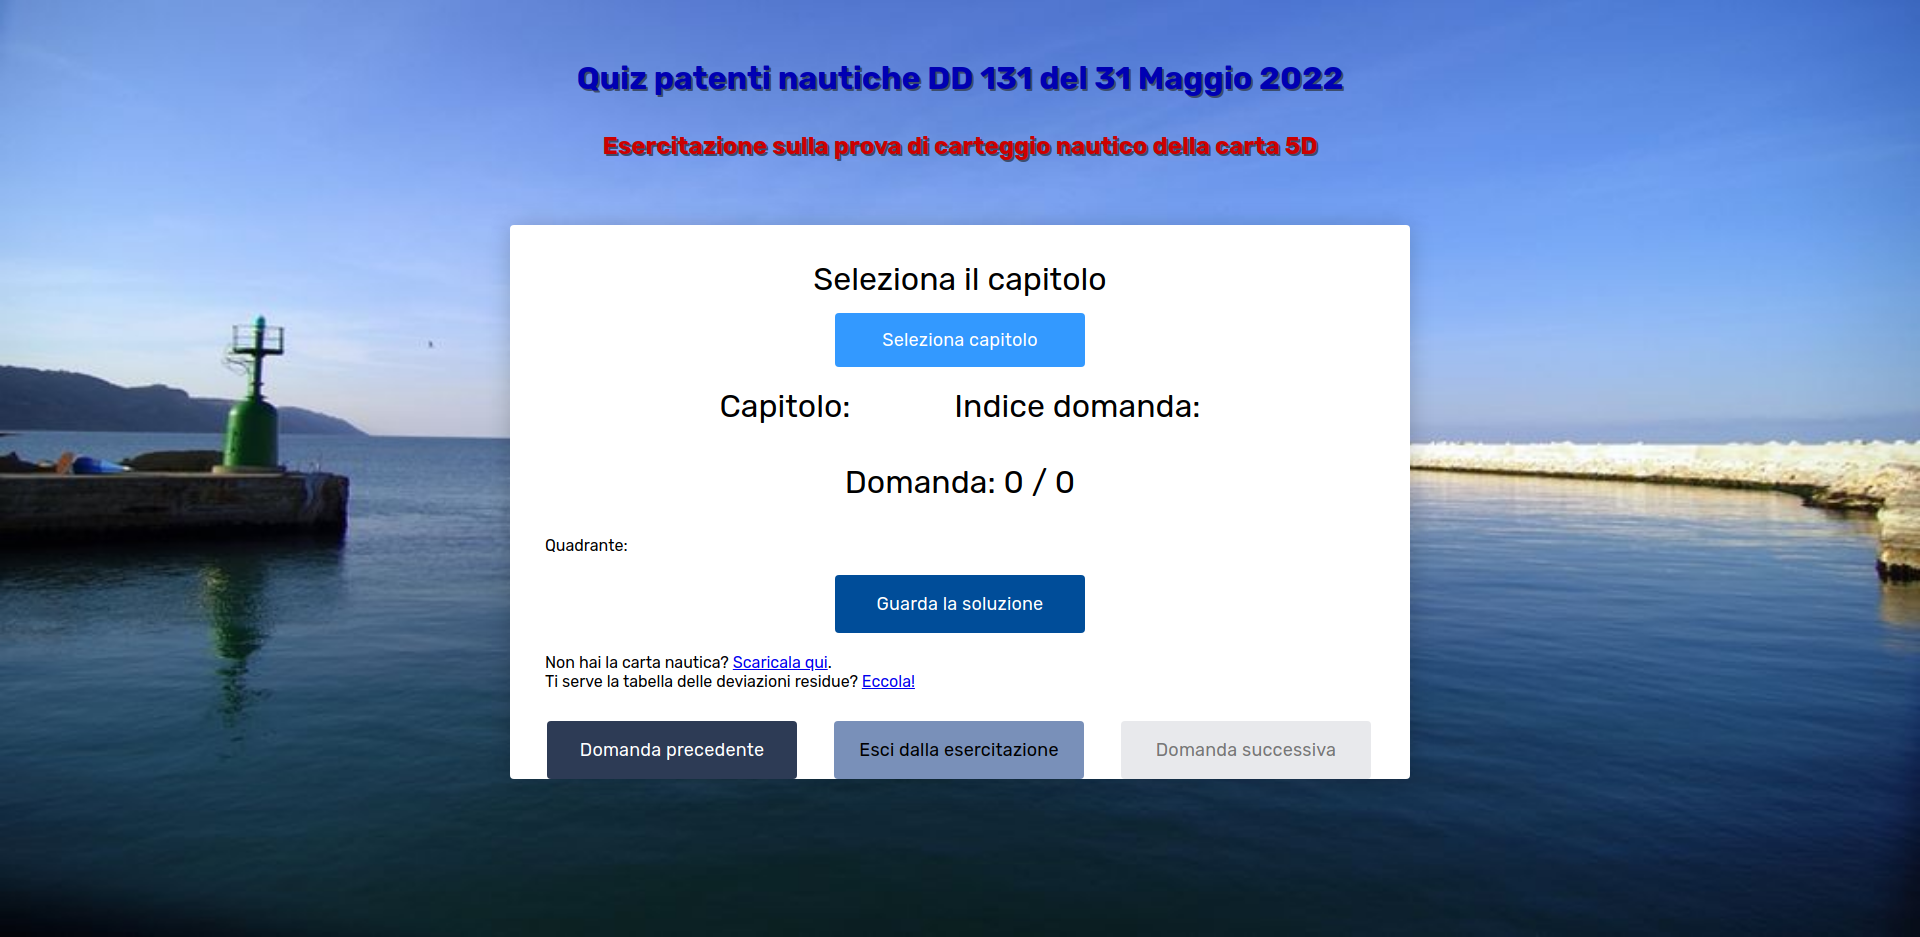
\includegraphics[scale=0.25]{Sites-images/20-Carteggio_5d.png}
		\caption{Pagina di carteggio sulla carta 5d.}
	\end{center}
\end{figure}

\begin{figure}[h]
	\begin{center}
		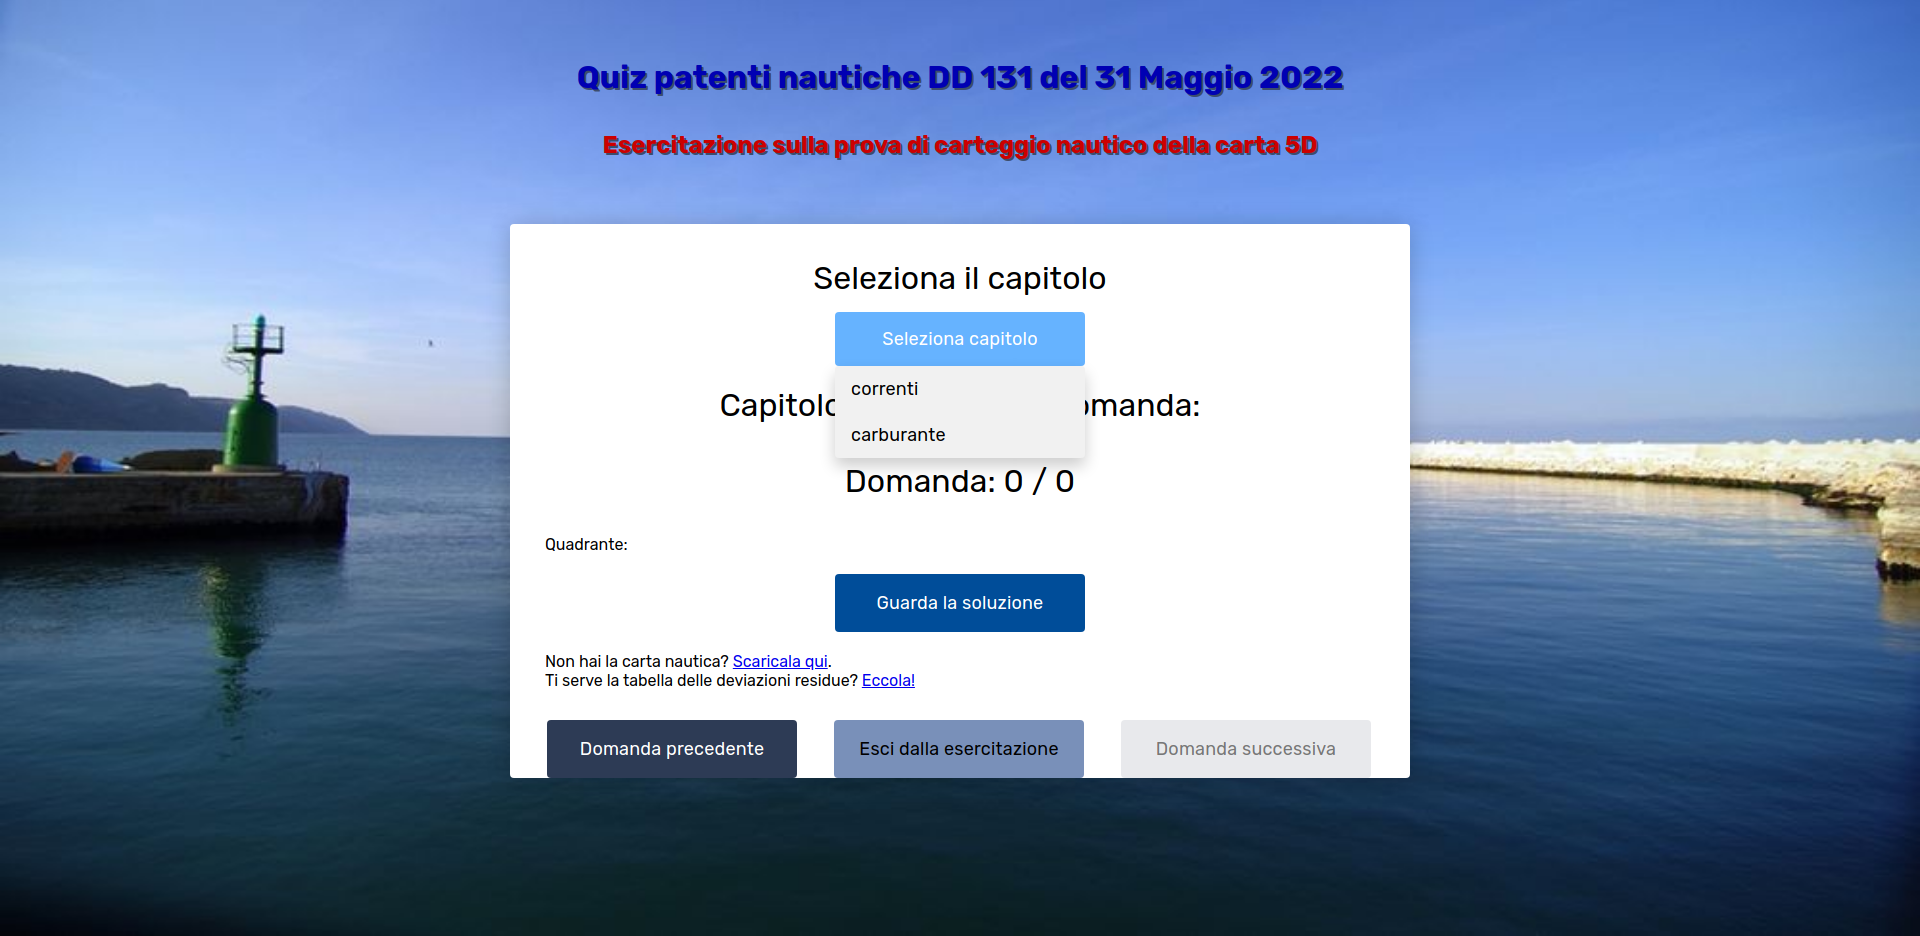
\includegraphics[scale=0.25]{Sites-images/21-Carteggio_5d_Selezione.png}
		\caption{Pagina di carteggio sulla carta 5d con selezione.}
	\end{center}
\end{figure}

\begin{figure}[h]
	\begin{center}
		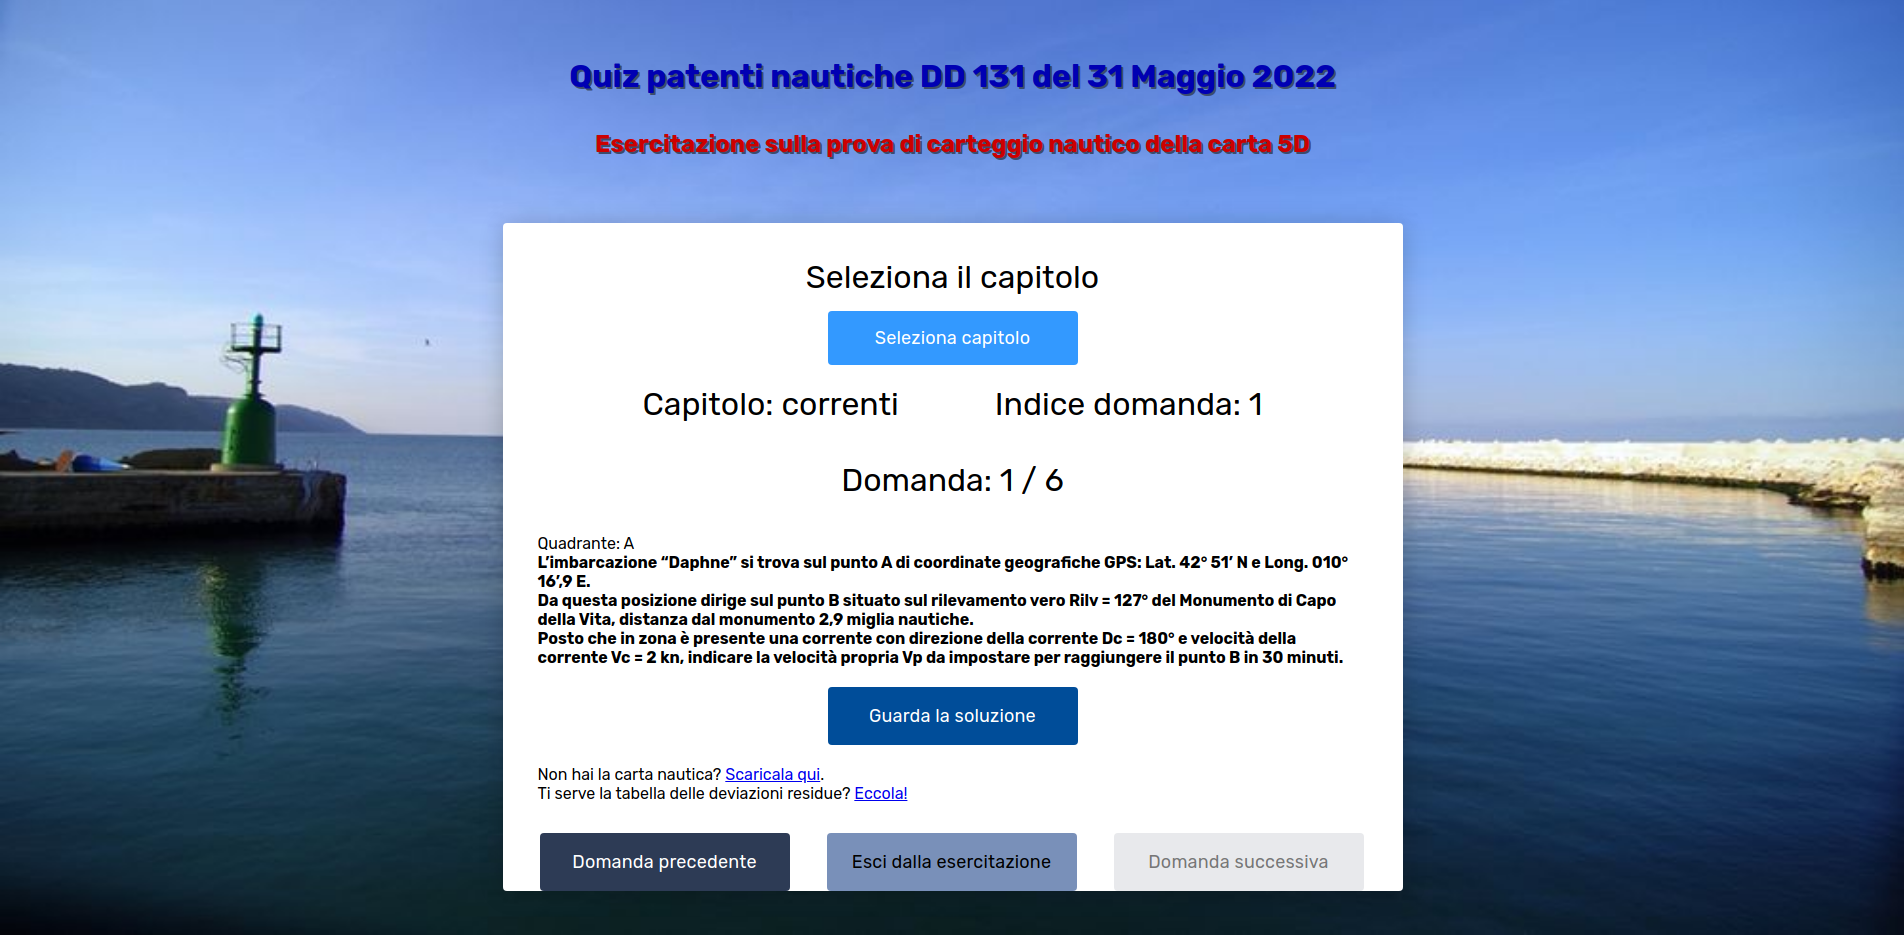
\includegraphics[scale=0.25]{Sites-images/22-Carteggio_5d_Domanda.png}
		\caption{Pagina di carteggio sulla carta 5d con la domanda.}
	\end{center}
\end{figure}

\begin{figure}[h]
	\begin{center}
		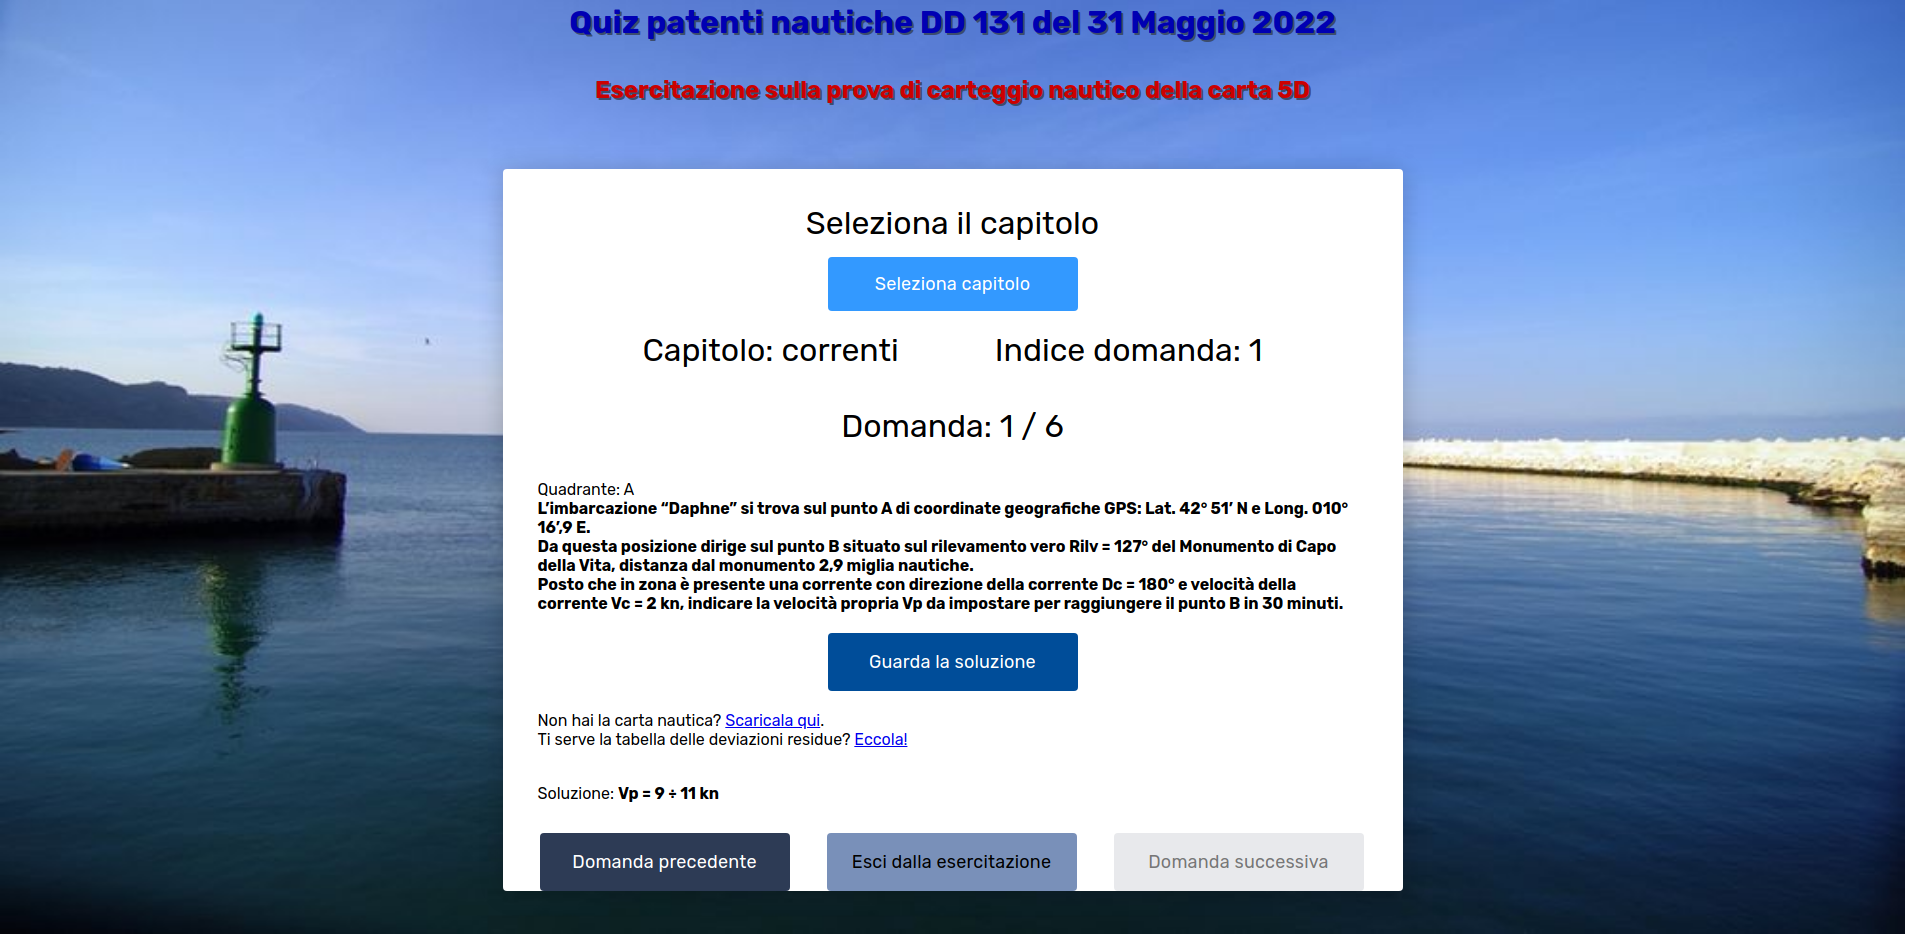
\includegraphics[scale=0.25]{Sites-images/23-Carteggio_5d_Risposta.png}
		\caption{Pagina di carteggio sulla carta 5d con la risposta.}
	\end{center}
\end{figure}

\textcolor{black}{Ora si passa alla presentazione delle parti salienti del codice della simulazione ed esercitazione per i quiz di base.}\\

\paragraph{\textcolor{black}{Simulazione quiz base}}\leavevmode\\

\textcolor{black}{Il codice che amministra questa simulazione è più complesso rispetto ai precedenti, per questa prova bisogna selezionare (in base al regolamento) una certa quantità di domande per ogni argomento ma per semplificare il database, le domande sono state inserite tutte nella stessa tabella e sono distinguibili attraverso l'argomento di appartenenza e dall'indice assoluto stabilito dal regolamento. Questa soluzione permette una manutenzione facilitata in caso di aggiornamento delle domande.\\
Però rende il codice più complesso, dovendo in primo luogo estrarre per ogni argomento il "range" tra gli indicici in cui fare la selezione causale delle domande.\\
Per questo motivo non verrà riportato tutto il codice, ma solo quello che mostra l'intera gestione delle domande di un singolo argomento, in modo da poter semplificare la lettura e la comprensione.}\\

\begin{lstlisting}[language=php]
	/*---------- EXTRACT QUESTIONS PROPERTIES ----------*/
	$query = $utilities->getMysql()->query("SELECT * FROM base_quiz_properties WHERE (id = '1')");
	$tempArray = $query->fetch_array(MYSQLI_ASSOC);
	
	$teoria_dello_scafo_questions                      = $tempArray['teoria_dello_scafo_questions'];
	$motori_questions                                  = $tempArray['motori_questions'];
	$sicurezza_della_navigazione_questions             = $tempArray['sicurezza_della_navigazione_questions'];
	$manovra_e_condotta_questions                      = $tempArray['manovra_e_condotta_questions'];
	$colreg_e_segnalamento_marittimo_questions         = $tempArray['colreg_e_segnalamento_marittimo_questions'];
	$meteorologia_questions                            = $tempArray['meteorologia_questions'];
	$navigazione_cartografica_ed_elettronica_questions = $tempArray['navigazione_cartografica_ed_elettronica_questions'];
	$normativa_diportistica_e_ambientale_questions     = $tempArray['normativa_diportistica_e_ambientale_questions'];
	$errors                                            = $tempArray['errors'];
	
	/*---------- FIND RANGE TO GENERATE QUESTIONS ----------*/
	$teoria_dello_scafo_questions_range = array();
	
	//---------- TEORIA DELLO SCAFO
	$query = $utilities->getMysql()->query("SELECT MIN(DISTINCT id) AS id FROM base_quiz WHERE (topic = 'TEORIA DELLO SCAFO')");
	$tempArray = $query->fetch_array(MYSQLI_ASSOC);
	$teoria_dello_scafo_questions_range['min'] = $tempArray['id'];
	$query = $utilities->getMysql()->query("SELECT MAX(DISTINCT id) AS id FROM base_quiz WHERE (topic = 'TEORIA DELLO SCAFO')");
	$tempArray = $query->fetch_array(MYSQLI_ASSOC);
	$teoria_dello_scafo_questions_range['max'] = $tempArray['id'];
	
	/*--------- PART TO GENERATE THE INDEXES AND TO CATCH THE QUESTIONS---------*/
	
	// variables where save indexes
	$indexNumbers = array();
	$questions = array();
	$indexQuestions = 0; //this will be increased after every question inserted.
	
	/---------- TEORIA DELLO SCAFO
	//-> $teoria_dello_scafo_questions
	//-> $teoria_dello_scafo_questions_range
	//-> teoria_dello_scafo
	$temp = 0;
	while($temp < $teoria_dello_scafo_questions){
		
		if($_SESSION['numbers']['teoria_dello_scafo'] !== null){
			// if i'm here meaning that the page has been reloaded
			if($indexNumbers['teoria_dello_scafo'][0] !== null){
				//generate number in recursive case
				$tempNum = random_int($teoria_dello_scafo_questions_range['min'], $teoria_dello_scafo_questions_range['max']);
				//verify that the number isn't duplicated
				while(in_array($tempNum,$indexNumbers['teoria_dello_scafo']) || in_array($tempNum,$_SESSION['numbers']['teoria_dello_scafo'])){
					$tempNum = random_int($teoria_dello_scafo_questions_range['min'], $teoria_dello_scafo_questions_range['max']);
				}
				
				//insert number
				$indexNumbers['teoria_dello_scafo'][$temp] = $tempNum;
				
			}else{
				//generate number on base case
				$tempNum = random_int($teoria_dello_scafo_questions_range['min'], $teoria_dello_scafo_questions_range['max']);
				//verify that the number is new (respect the past)
				while(in_array($tempNum,$_SESSION['numbers']['teoria_dello_scafo'])){
					$tempNum = random_int($teoria_dello_scafo_questions_range['min'], $teoria_dello_scafo_questions_range['max']);
				}
				//insert number
				$indexNumbers['teoria_dello_scafo'][$temp] = $tempNum;
			}
			
		}else{
			//if i'm here meaning that the page is new
			if($indexNumbers['teoria_dello_scafo'][0] !== null){
				//generate number in recursive case
				$tempNum = random_int($teoria_dello_scafo_questions_range['min'], $teoria_dello_scafo_questions_range['max']);
				//verify that the number isn't duplicated
				while(in_array($tempNum,$indexNumbers['teoria_dello_scafo'])){
					$tempNum = random_int($teoria_dello_scafo_questions_range['min'], $teoria_dello_scafo_questions_range['max']);
				}
				
				//insert number
				$indexNumbers['teoria_dello_scafo'][$temp] = $tempNum;
				
			}else{
				//generate number on base case
				$indexNumbers['teoria_dello_scafo'][$temp] = random_int($teoria_dello_scafo_questions_range['min'], $teoria_dello_scafo_questions_range['max']);
			}
		}
		/*catch question*/
		$query = $utilities->getMysql()->query("SELECT * FROM base_quiz WHERE (id = '{$indexNumbers['teoria_dello_scafo'][$temp]}')");
		$tempArray = $query->fetch_array(MYSQLI_ASSOC);
		$questions[$indexQuestions] = $tempArray;
		++$indexQuestions;
		
		++$temp;
		}
		
		$_SESSION['numbers'] = $indexNumbers;
		
		// get current number of loaded questions
		$totalQuestions = count($questions);
		
		/*--------- PREPARE ARRAY WITH ANSWER FOR CHECKING PART IN JS---------*/
		$questionsAnswers = array();
		
		$temp = 0;
		while($temp < $totalQuestions){
			
			$questionsAnswers[$temp]['answer_1'] = $questions[$temp]['answer_1'];
			$questionsAnswers[$temp]['answer_2'] = $questions[$temp]['answer_2'];
			$questionsAnswers[$temp]['answer_3'] = $questions[$temp]['answer_3'];
			
			++$temp;
		}
\end{lstlisting}
\textcolor{black}{Si può notare che la logica di fondo non è stata stravolta ma è stata adeguata al specifico caso, infatti, come anche in precedenza, le domande sono state tutte inserite in un "array" comune e l'inserimento è stato fatto come di consueto alla fine dei cicli "while" annidati per poter risparmiare risorse. La novità principale in questo caso risiede nel sistema un pochino più complesso di selezione delle domande.\\
Rispetto al passato dove la risposta alle domande era aperta (siccome nel lavorare con le carte nautiche è facile commettere degli errori di misurazione meccanici) qui l'utente deve selezionare la risposta che ritiene giusta rispetto alle tre proposte. Viene quindi riportato inferiormente la parte di codice "html" che mostra come è stata costruita la visualizzazione delle domande.}\\

\begin{lstlisting}[language=html]
	<?php
	/*--------- GENERATE QUESTIONS---------*/
	$temp = 0;
	while($temp < $totalQuestions){
		
		
		//prepare variables
		$answers_1 = null;
		$answers_2 = null;
		$answers_3 = null;
		
		//--------- generate the check's answers with truth properties ----------
		
		//first answer case
		if($questions[$temp]['answer_1'] == 'V'){
			$answers_1 = "
			<div class='answer1' id='answer1".$temp."' style='color: green'> V-> ".$questions[$temp]['answer_text_1']." </div>
			<div class='answer1_null' id='answer1_null".$temp."' > V-> ".$questions[$temp]['answer_text_1']." </div>
			";
		}else{
			$answers_1 = "
			<div class='answer1' id='answer1".$temp."' style='color: red'> F-> ".$questions[$temp]['answer_text_1']." </div>
			<div class='answer1_null' id='answer1_null".$temp."' > F-> ".$questions[$temp]['answer_text_1']." </div>
			";
		}
		
		//second answer case
		if($questions[$temp]['answer_2'] == 'V'){
			$answers_2 = "
			<div class='answer2' id='answer2".$temp."' style='color: green'> V-> ".$questions[$temp]['answer_text_2']." </div>
			<div class='answer2_null' id='answer2_null".$temp."' > V-> ".$questions[$temp]['answer_text_2']." </div>
			";
		}else{
			$answers_2 = "
			<div class='answer2' id='answer2".$temp."' style='color: red'> F-> ".$questions[$temp]['answer_text_2']." </div>
			<div class='answer2_null' id='answer2_null".$temp."' > F-> ".$questions[$temp]['answer_text_2']." </div>
			";
		}
		
		//thirth answer case
		if($questions[$temp]['answer_3'] == 'V'){
			$answers_3 = "
			<div class='answer3' id='answer3".$temp."' style='color: green'> V-> ".$questions[$temp]['answer_text_3']." </div>
			<div class='answer3_null' id='answer3_null".$temp."' > V-> ".$questions[$temp]['answer_text_3']." </div>
			";
		}else{
			$answers_3 = "
			<div class='answer3' id='answer3".$temp."' style='color: red'> F-> ".$questions[$temp]['answer_text_3']." </div>
			<div class='answer3_null' id='answer3_null".$temp."' > F-> ".$questions[$temp]['answer_text_3']." </div>
			";
		}
		
		
		//--------- PRINT QUESTION ----------
		$tempImg = null;
		if($questions[$temp]['img'] !== null){
			$tempImg = "<div class='answerImg' id='answerImg".$temp."'> <img src='data:image/jpeg;base64,".base64_encode($questions[$temp]['img'])."'/> </div>";
		}
		echo "<div class='question'>
		<p><b> ".$questions[$temp]['question_text']." </b></p>
		".$tempImg."
		<div id= 'answerRadios'>
		<div class='label1' id='label1".$temp."'> <label> <input type='radio' name='radio".$temp."' id='radio1".$temp."' > ".$questions[$temp]['answer_text_1']." </label> </div>
		<div class='label2' id='label2".$temp."'> <label> <input type='radio' name='radio".$temp."' id='radio2".$temp."' > ".$questions[$temp]['answer_text_2']." </label> </div>
		<div class='label3' id='label3".$temp."'> <label> <input type='radio' name='radio".$temp."' id='radio3".$temp."' > ".$questions[$temp]['answer_text_3']." </label> </div>
		</div>
		".$answers_1."
		".$answers_2."
		".$answers_3."
		</div>";
		
		++$temp;
	}
	?>
	</div>
	<div class="actions">
	<input type='button' name='revision' value='Verifica le risposte' id='revision' onclick='check()'/>
	</div>
\end{lstlisting}

\textcolor{black}{Per prima cosa sono state preparate in delle variabili le "stringhe di codice html" per ogni risposta, in modo da riferirsi successivamente a queste in una forma più compatta e chiara. Vi è la parte di codice che effettivamente "stampa" le domande con le relative risposte (la fase di prima è propedeutica per evitare di complicare questa porzione). Per raccogliere la risposta dell'utente si è usato l'oggetto "radio" (dei quali ne è selezionabile solo uno per domanda) rispetto ai classici pulsanti.\\ 
La correzione del codice è delegata alla parte in "javascript", qui riportato inferiormente.}\\

\begin{lstlisting}[language=java]
	<script>
	
	/*--------- PREPARE IMPORT FIELDS---------*/
	var errors    = 0;
	var corrected = false;
	
	/*--------- GET IMPORTANT FIELDS FROM PHP---------*/
	var maxErrors = <?php echo $errors;?>;
	//the array with all answers
	var questionsAnswers = JSON.parse(<?php echo "'".json_encode($questionsAnswers)."'"; ?>);
	var totalQuestions = <?php echo $totalQuestions;?>;
	
	/*--------- HIDE THE ELEMENTS AT THE BEGINNING---------*/
	var temp = 0;
	
	while(temp < totalQuestions){
		var answer1      = document.getElementById("answer1"+temp);
		var answer1_null = document.getElementById("answer1_null"+temp);
		var answer2      = document.getElementById("answer2"+temp);
		var answer2_null = document.getElementById("answer2_null"+temp);
		var answer3      = document.getElementById("answer3"+temp);
		var answer3_null = document.getElementById("answer3_null"+temp);
		
		answer1.style.display      = "none";
		answer1_null.style.display = "none";
		answer2.style.display      = "none";
		answer2_null.style.display = "none";
		answer3.style.display      = "none";
		answer3_null.style.display = "none";
		
		++temp;
	}
	
	var passed    = document.getElementById("passed");
	var notpassed = document.getElementById("notpassed");
	
	passed.style.display    = "none";
	notpassed.style.display = "none";
	
	/*--------- CHECKING FUNCTION---------*/
	function check(){
		
		temp = 0;
		while(temp < totalQuestions && !corrected){
			
			// hide common fields
			var label1       = document.getElementById("label1"+temp);
			var label2       = document.getElementById("label2"+temp);
			var label3       = document.getElementById("label3"+temp);
			
			label1.style.display = "none";
			label2.style.display = "none";
			label3.style.display = "none";
			
			//GIVEN ANSWER 1
			if(document.getElementById(String('radio1'+temp)).checked){
				
				//show answer
				var answer1      = document.getElementById("answer1"+temp);
				var answer2_null = document.getElementById("answer2_null"+temp);
				var answer3_null = document.getElementById("answer3_null"+temp);
				
				answer1.style.display         = "block";
				answer2_null.style.display    = "block";
				answer3_null.style.display    = "block";
				
				//count error
				if(questionsAnswers[temp]['answer_1']!== 'V'){
					++errors;
				}
				
			}else{
				//GIVEN ANSWER 2
				if(document.getElementById(String('radio2'+temp)).checked){
					
					//show answer
					var answer1_null = document.getElementById("answer1_null"+temp);
					var answer2      = document.getElementById("answer2"+temp);
					var answer3_null = document.getElementById("answer3_null"+temp);
					
					answer1_null.style.display    = "block";
					answer2.style.display         = "block";
					answer3_null.style.display    = "block";
					
					//count error
					if(questionsAnswers[temp]['answer_2']!== 'V'){
						++errors;
					}
					
				}else{
					//GIVEN ANSWER 3
					if(document.getElementById(String('radio3'+temp)).checked){
						
						//show answer
						var answer1_null = document.getElementById("answer1_null"+temp);
						var answer2_null = document.getElementById("answer2_null"+temp);
						var answer3      = document.getElementById("answer3"+temp);
						
						answer1_null.style.display    = "block";
						answer2_null.style.display    = "block";
						answer3.style.display         = "block";
						
						//count error
						if(questionsAnswers[temp]['answer_3']!== 'V'){
							++errors;
						}
						
					}else{
						//NULL ANSWER CASE
						
						//show answer
						var answer1_null = document.getElementById("answer1_null"+temp);
						var answer2_null = document.getElementById("answer2_null"+temp);
						var answer3_null = document.getElementById("answer3_null"+temp);
						
						answer1_null.style.display    = "block";
						answer2_null.style.display    = "block";
						answer3_null.style.display    = "block";
						
						//count error
						++errors;
						
					}
				}
			}
			
			// end while cycle
			++temp;
		}
		
		//set that the correction has happened
		corrected = true;
		
		if(errors < maxErrors){
			
			passed.style.display = "block";
			
		}else{
			
			notpassed.style.display = "block";
		}
		
	}
\end{lstlisting}\leavevmode\\

\textcolor{black}{In questa situazione, nella fase di preparazione dell'operazione di correzione è stato necessario passare delle informazione dal "back-end" (quindi della parte di codice "php") al "front-end" (in questo caso la parte in "javascript"). Purtroppo questa cosa è stata fatta "in chiaro" (quindi in modo poco elegante) serializzando le informazioni tramite il sistema "JSON" al posto di "AJAX" che, si presuppone a causa di alcune chiamate a sistema sbagliate, non ha mai funzionato. Si pensa che siano le chiamate a sistema a fallire siccome durante le prove, il terminale non riportava alcun errore, anzi, se si attivavano le stampe per il "debug" venivano visualizzati dei messaggi che comunicavano esito positivo, anche se alla fine ciò non risultava.\\
Finita la fase di preparazione, si oscurano tutte le risposte e il messaggio che dice se la prova è stata più o meno superata. Successivamente è stata scritta la funzione che si occupa di eseguire la correzione delle risposte, in questo caso una caratteristica fondamentale è quella di mostrare la risposta data e quella corretta. La correzione viene fatta sostituendo tutti i pulsanti "radio" con la lettera V oppure F a seconda se la riposta adiacente sia vera oppure falsa, la risposta data dall'utente viene evidenziata cambiando il colore del testo della risposta, in verde nel caso in cui l'utente abbia scelto la risposta giusta e in rosso nel caso contrario. Ogni risposta errata farà aumentare il contatore degli errori con il quale si determina poi se l'utente ha superato o meno la simulazione. La scritta che comunica o meno il superamento della prova viene fatta comparire alla fine della correzione.}\\

\begin{figure}[h]
	\begin{center}
		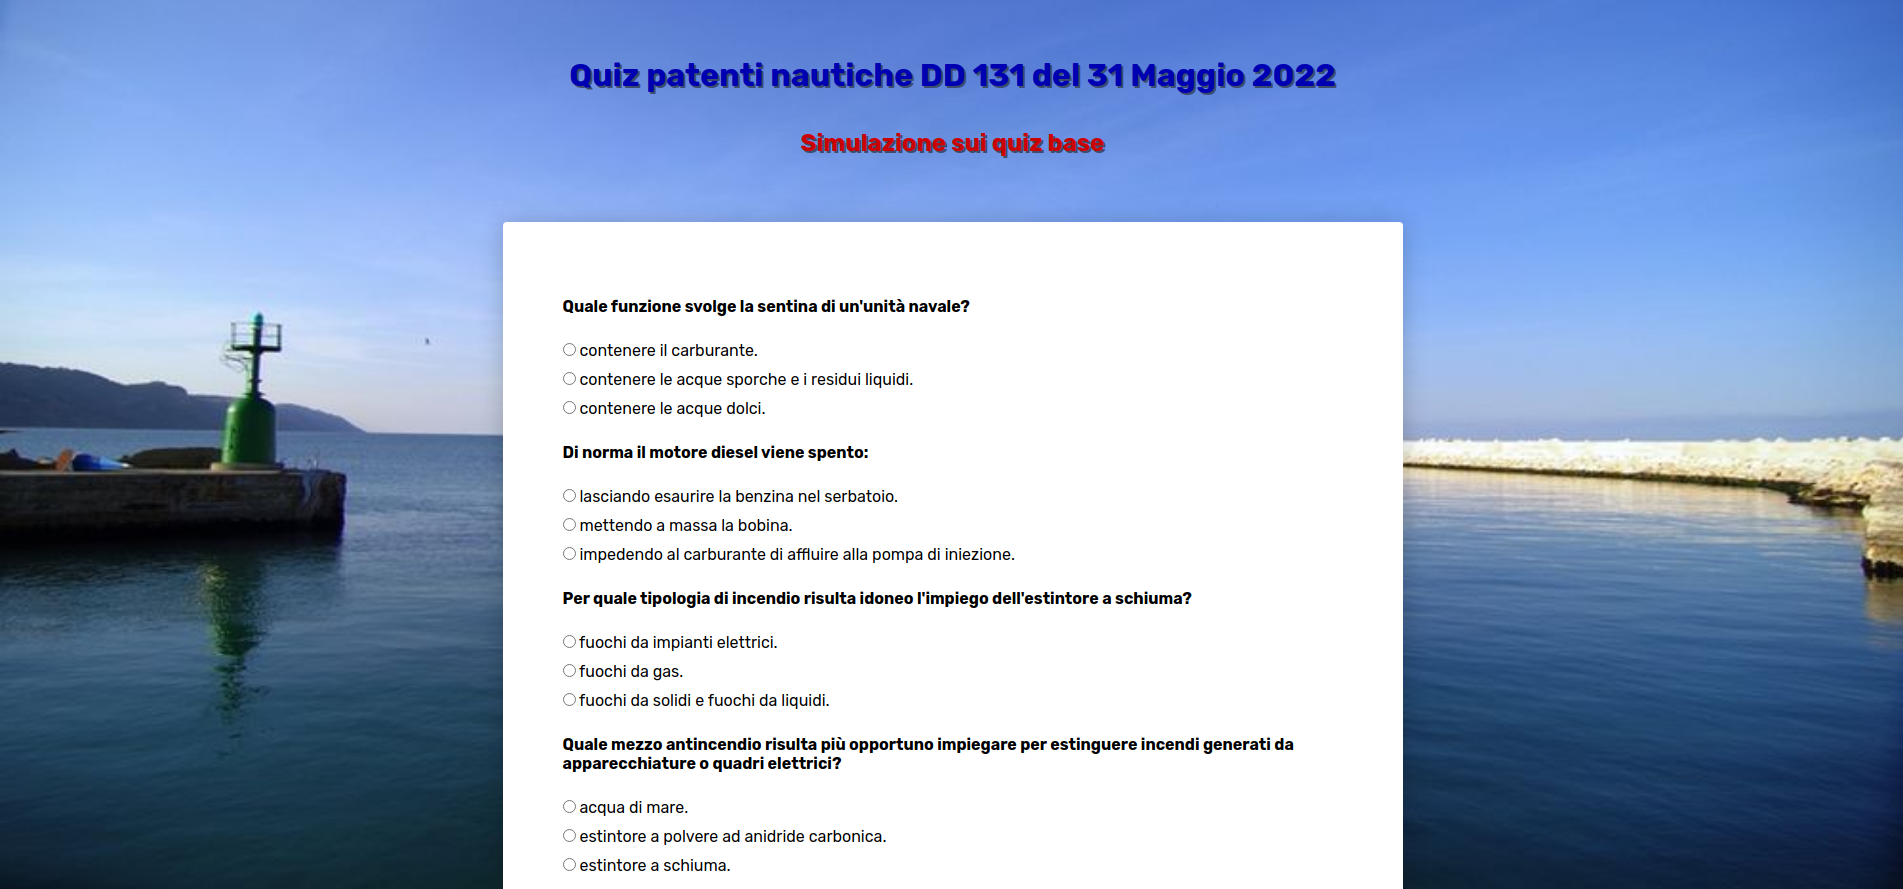
\includegraphics[scale=0.25]{Sites-images/28-Simulazione_quiz_base1.png}
		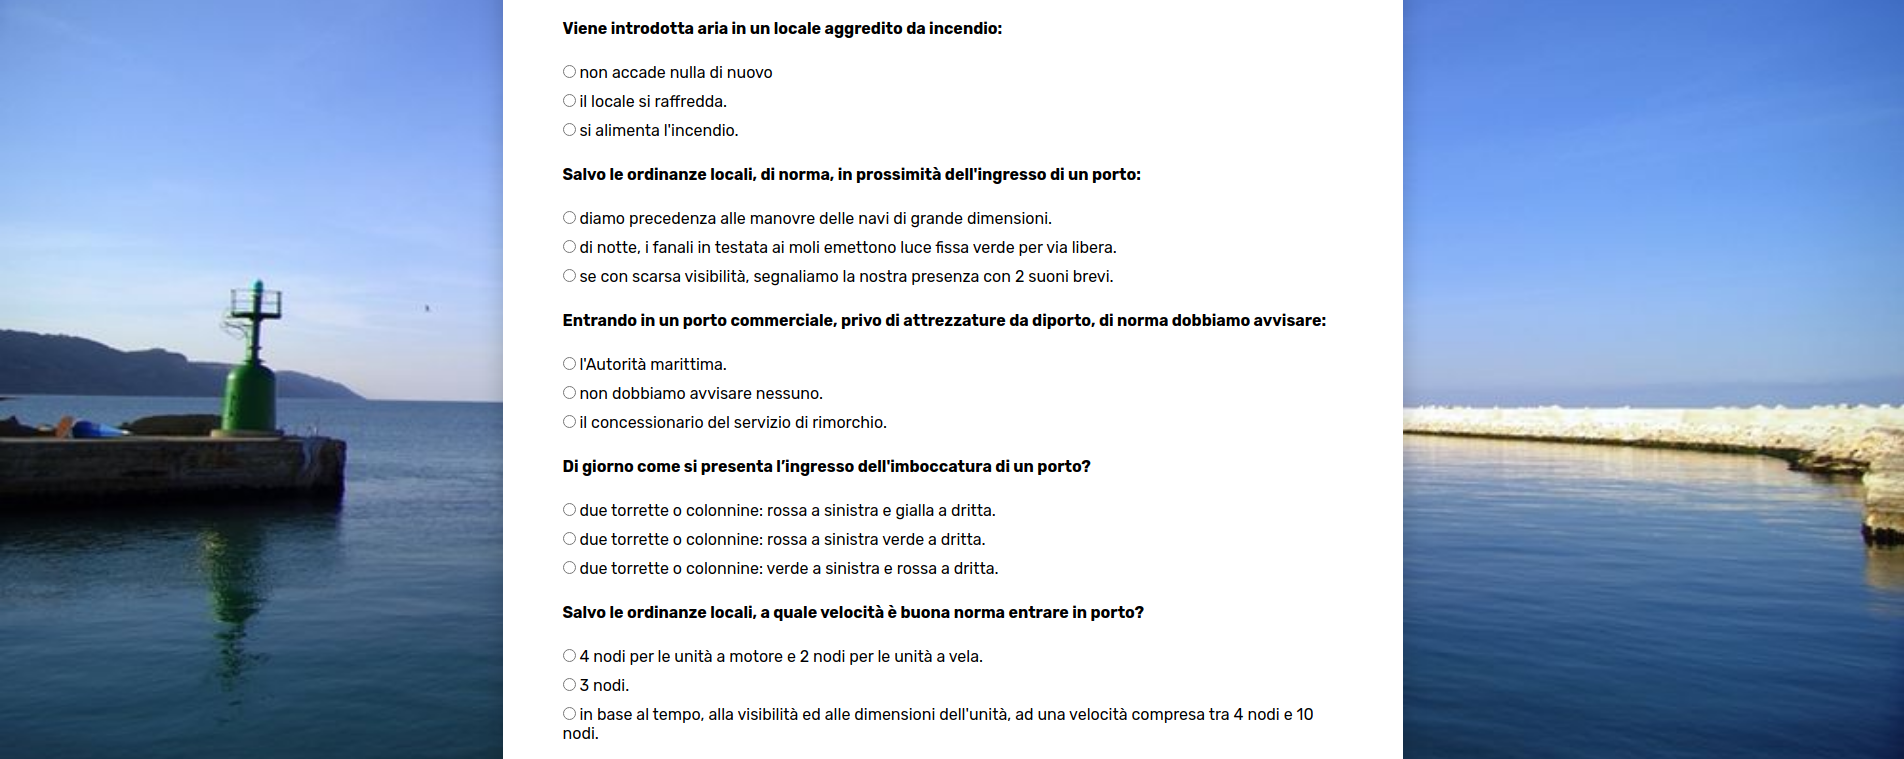
\includegraphics[scale=0.25]{Sites-images/29-Simulazione_quiz_base2.png}
		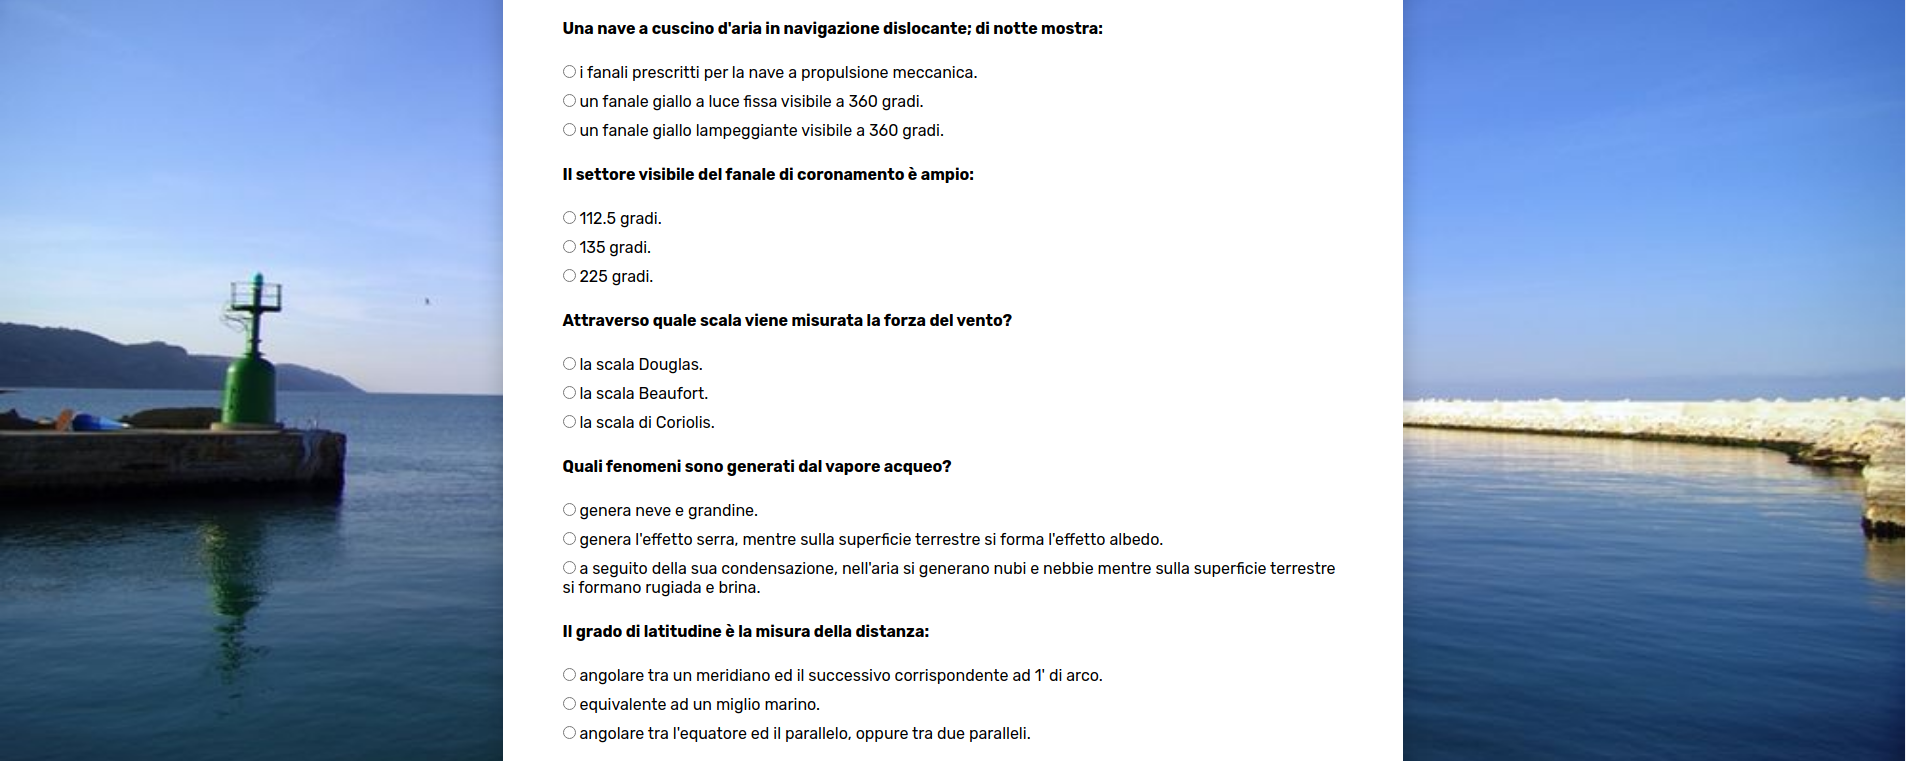
\includegraphics[scale=0.25]{Sites-images/30-Simulazione_quiz_base3.png}
		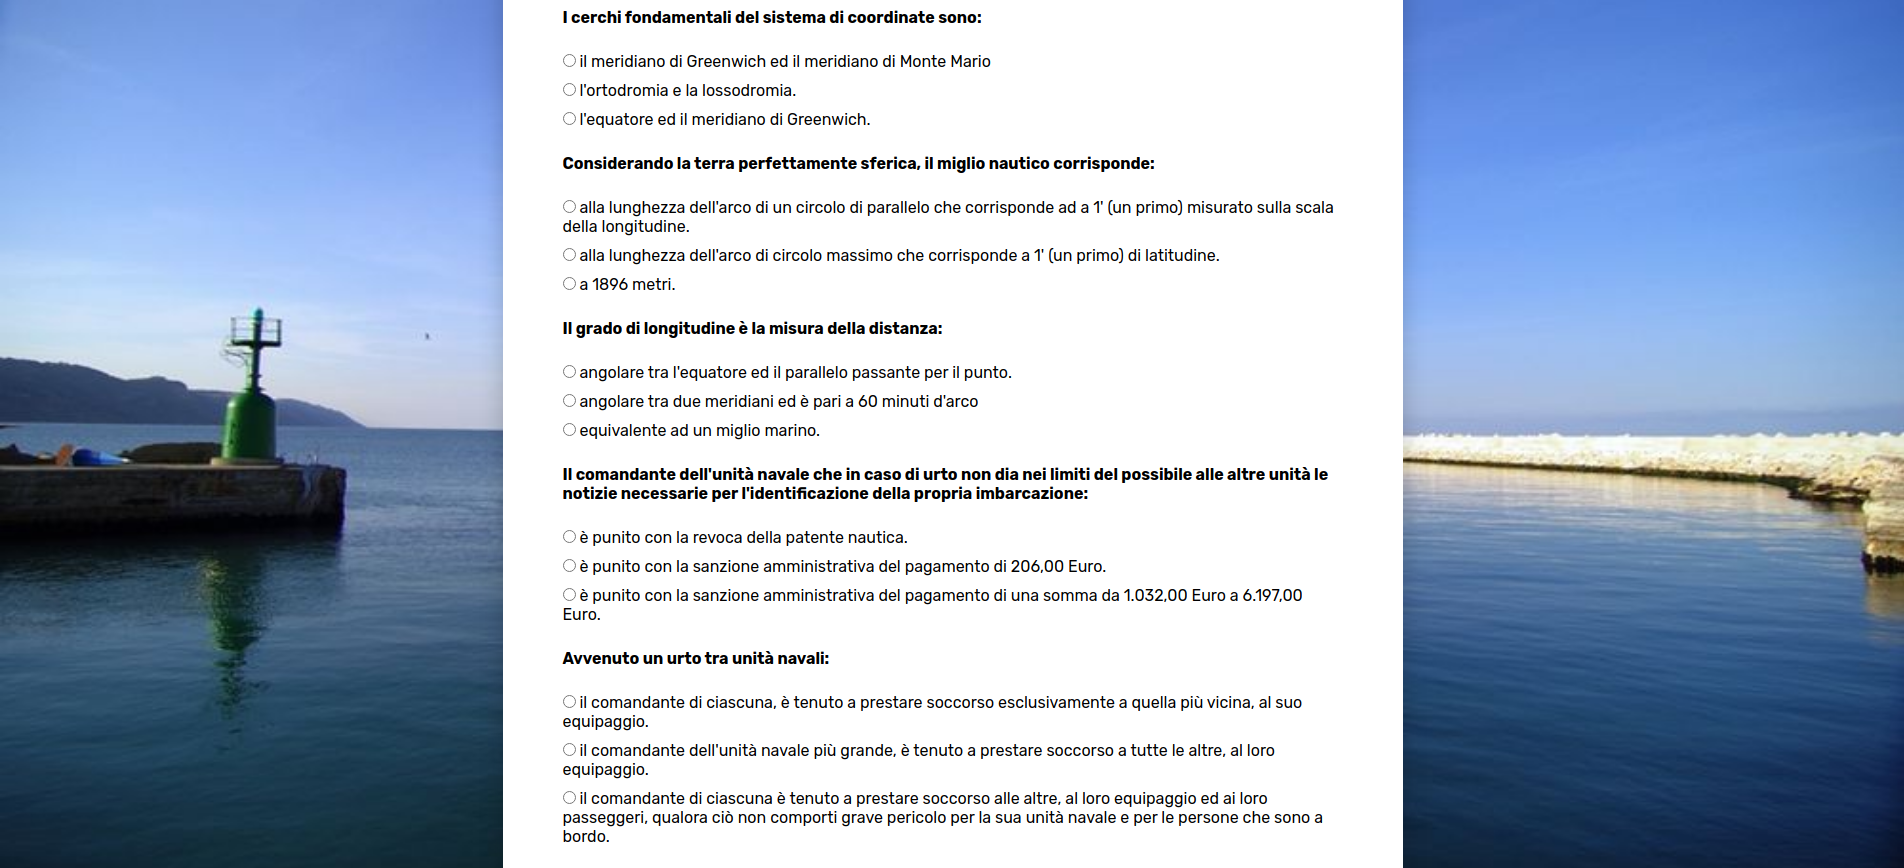
\includegraphics[scale=0.25]{Sites-images/31-Simulazione_quiz_base4.png}
		
\includegraphics[scale=0.25]{Sites-images/32-Simulazione_quiz_base5.png}
		\caption{Pagina di simulazione dei quiz base.}
		(Ricomposta)
	\end{center}
\end{figure}

\begin{figure}[h]
	\begin{center}
		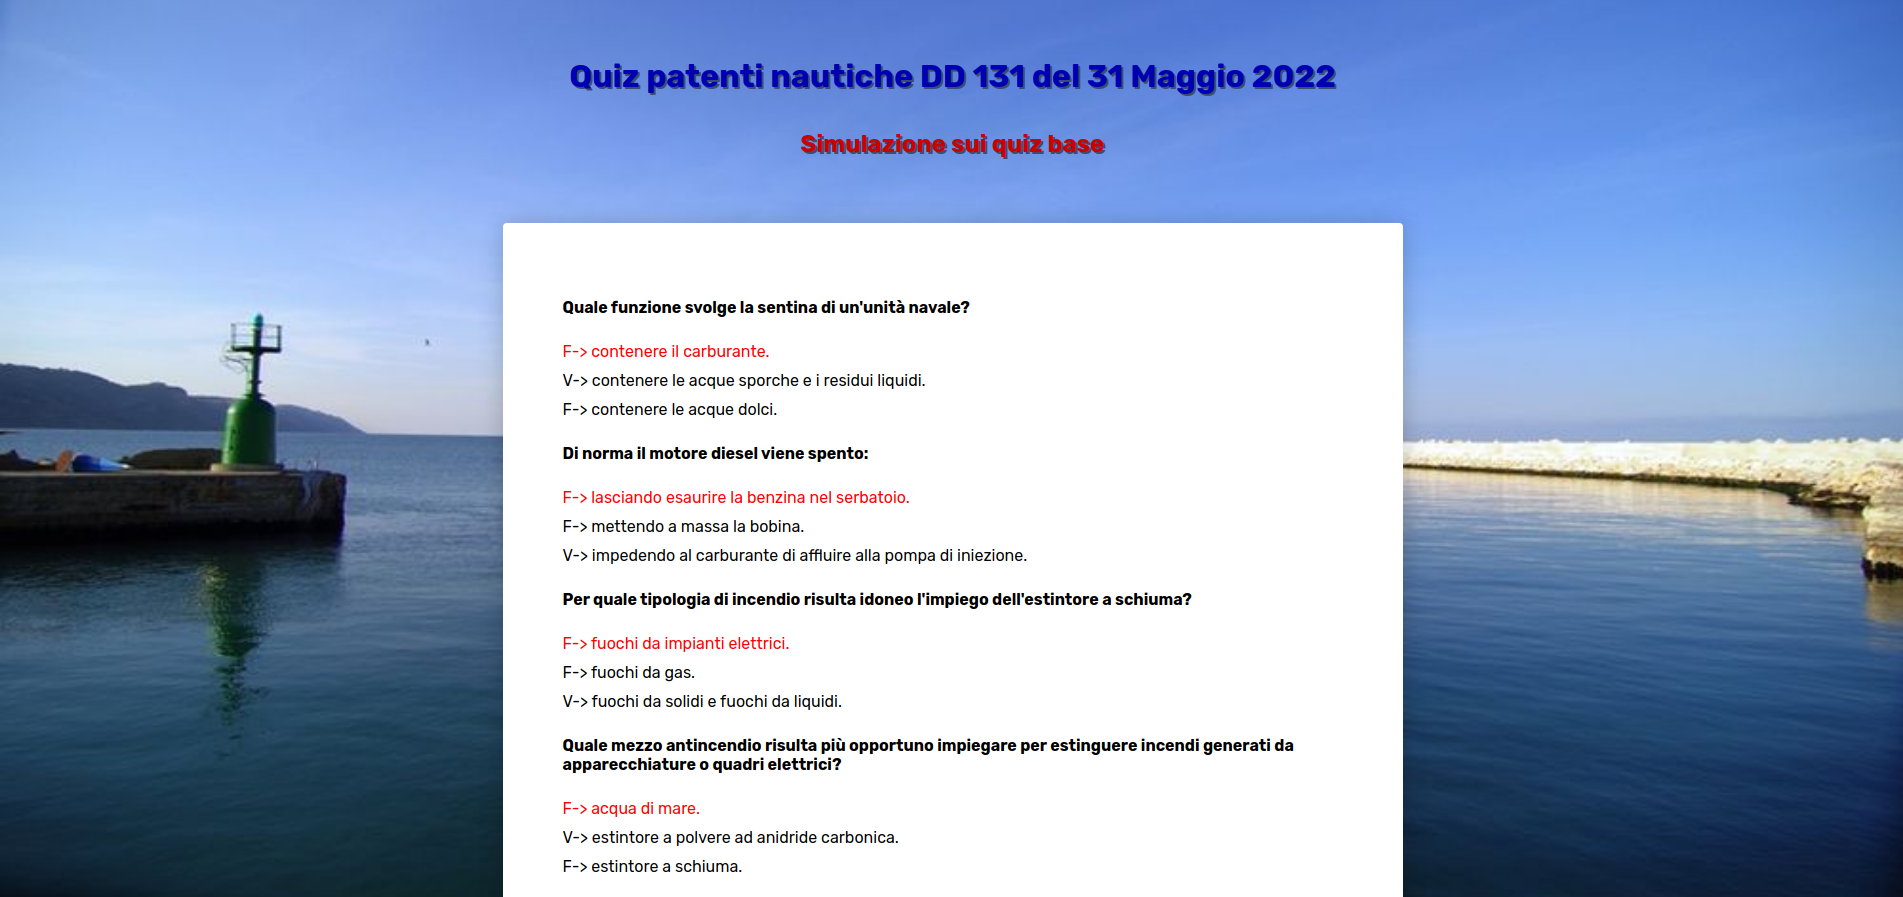
\includegraphics[scale=0.25]{Sites-images/33-Simulazione_quiz_base-risposte1.png}
		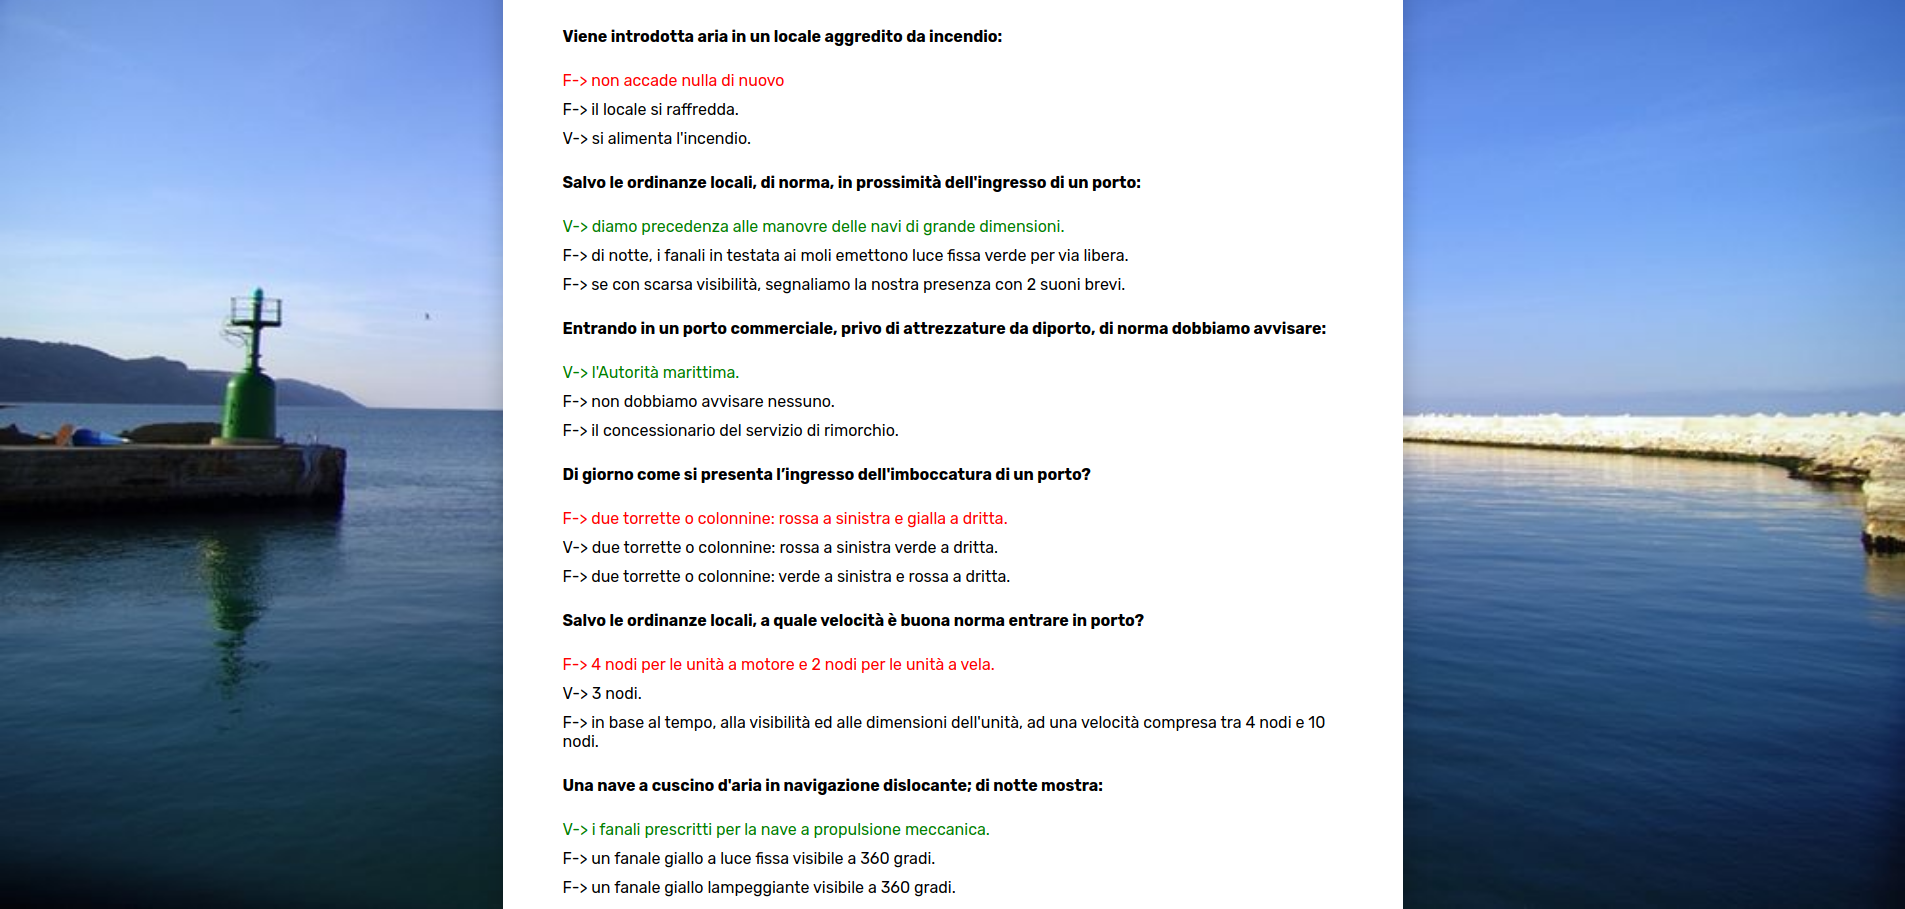
\includegraphics[scale=0.25]{Sites-images/34-Simulazione_quiz_base-risposte2.png}
		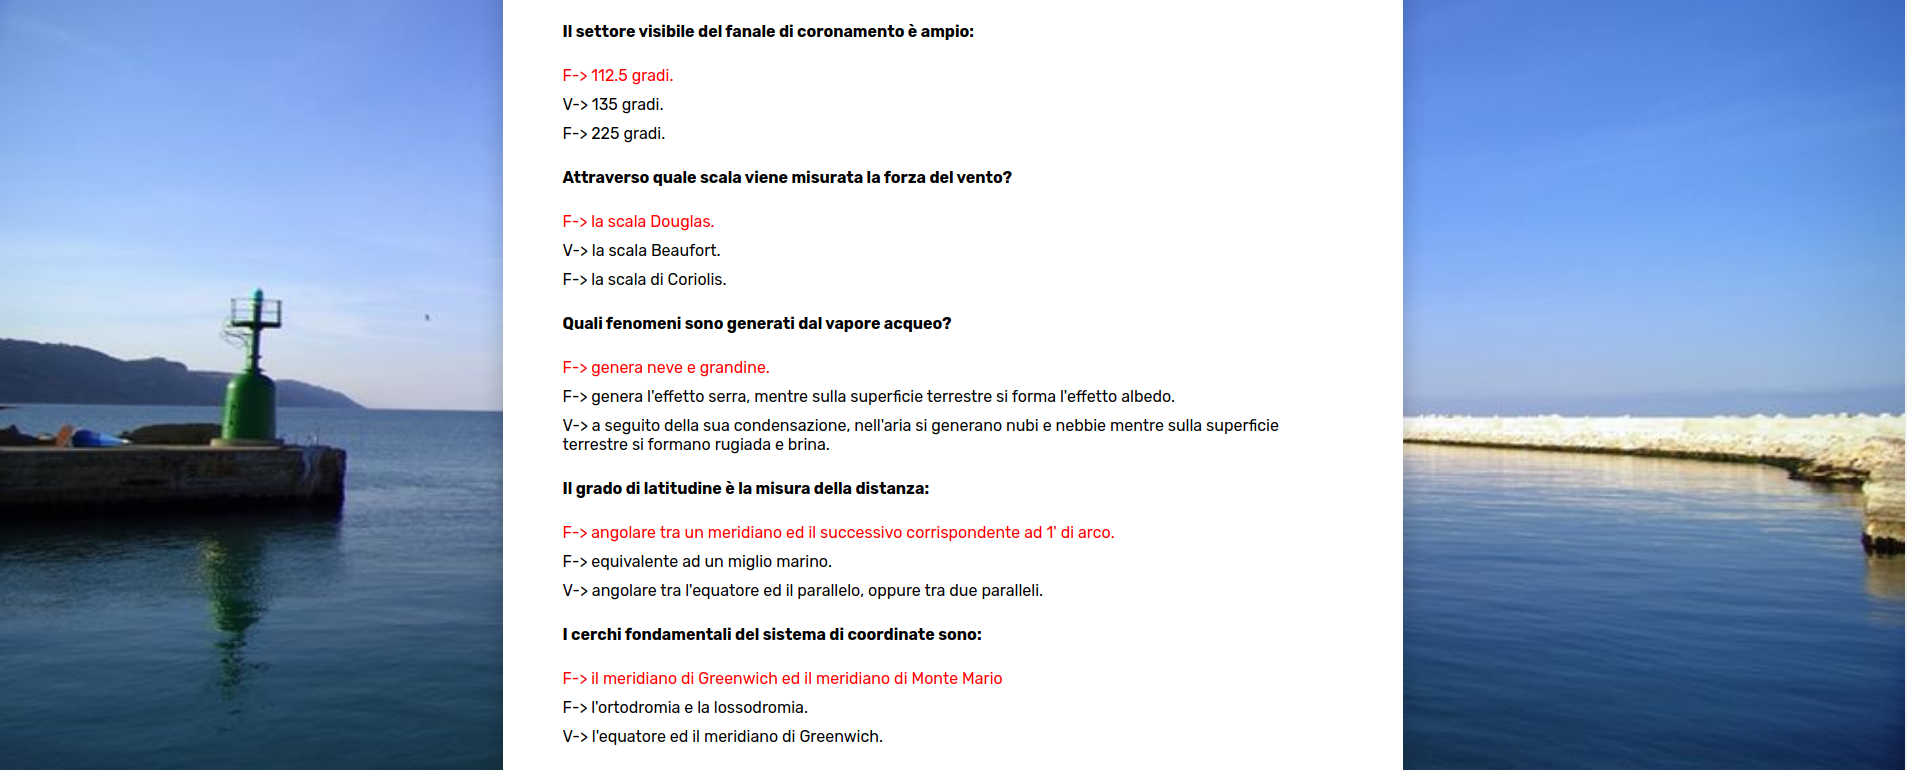
\includegraphics[scale=0.25]{Sites-images/35-Simulazione_quiz_base-risposte3.png}
		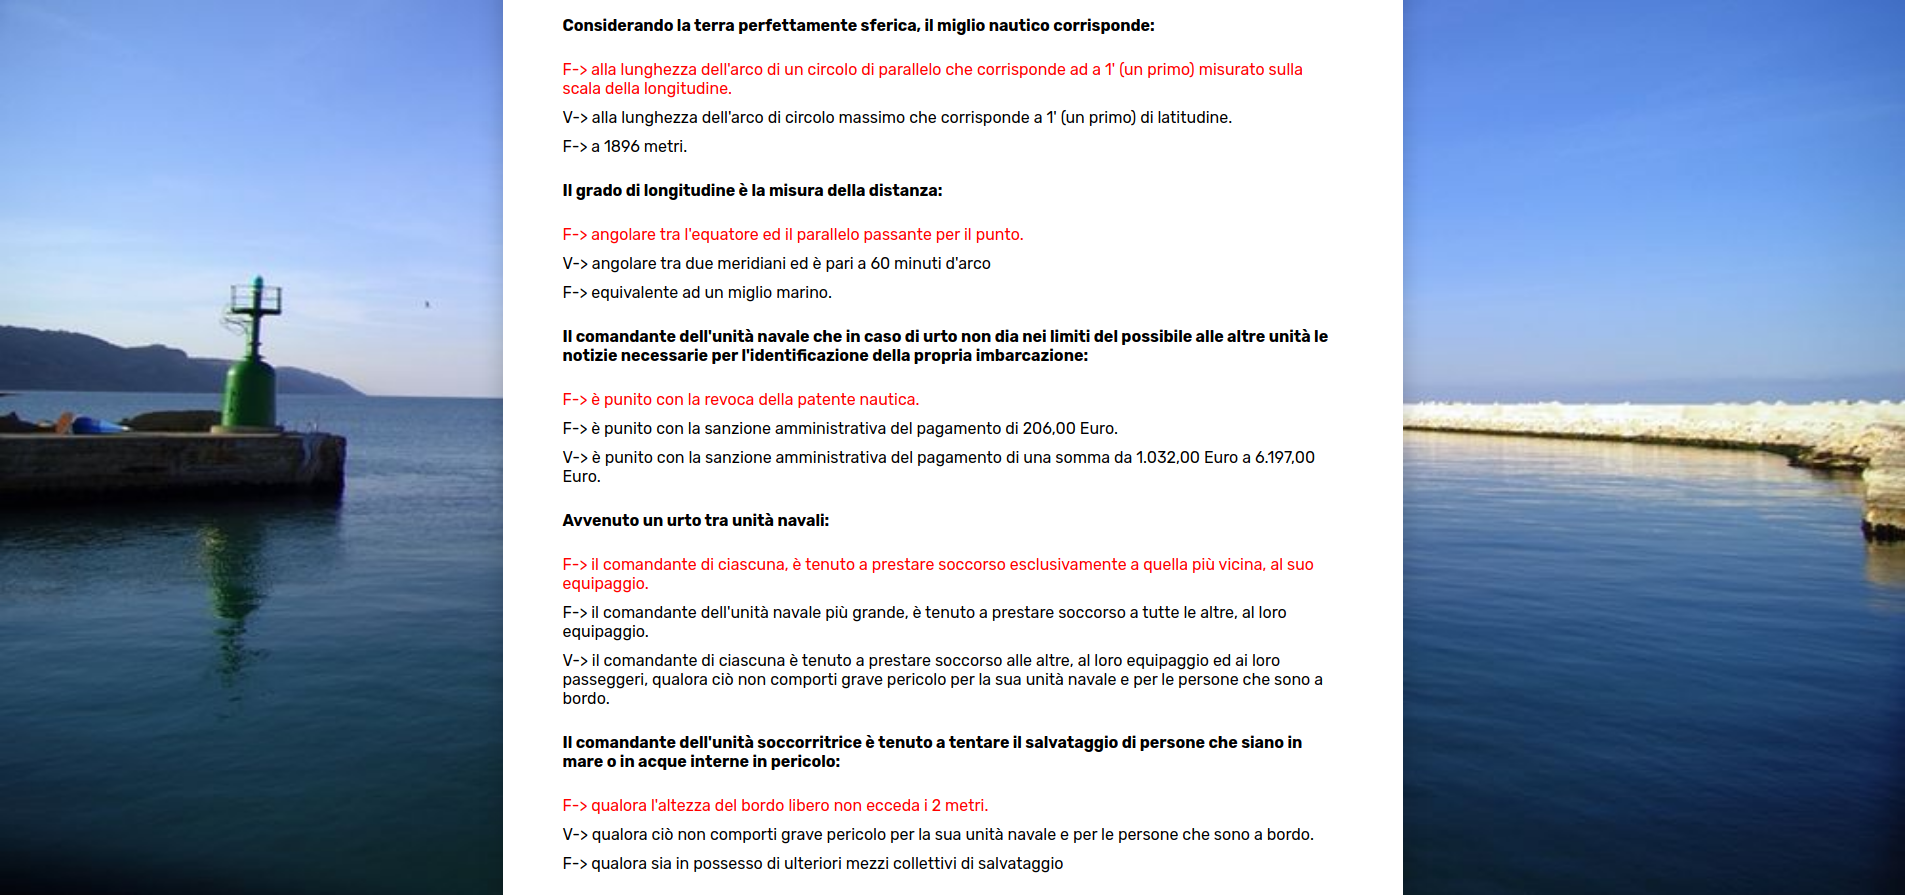
\includegraphics[scale=0.25]{Sites-images/36-Simulazione_quiz_base-risposte4.png}
		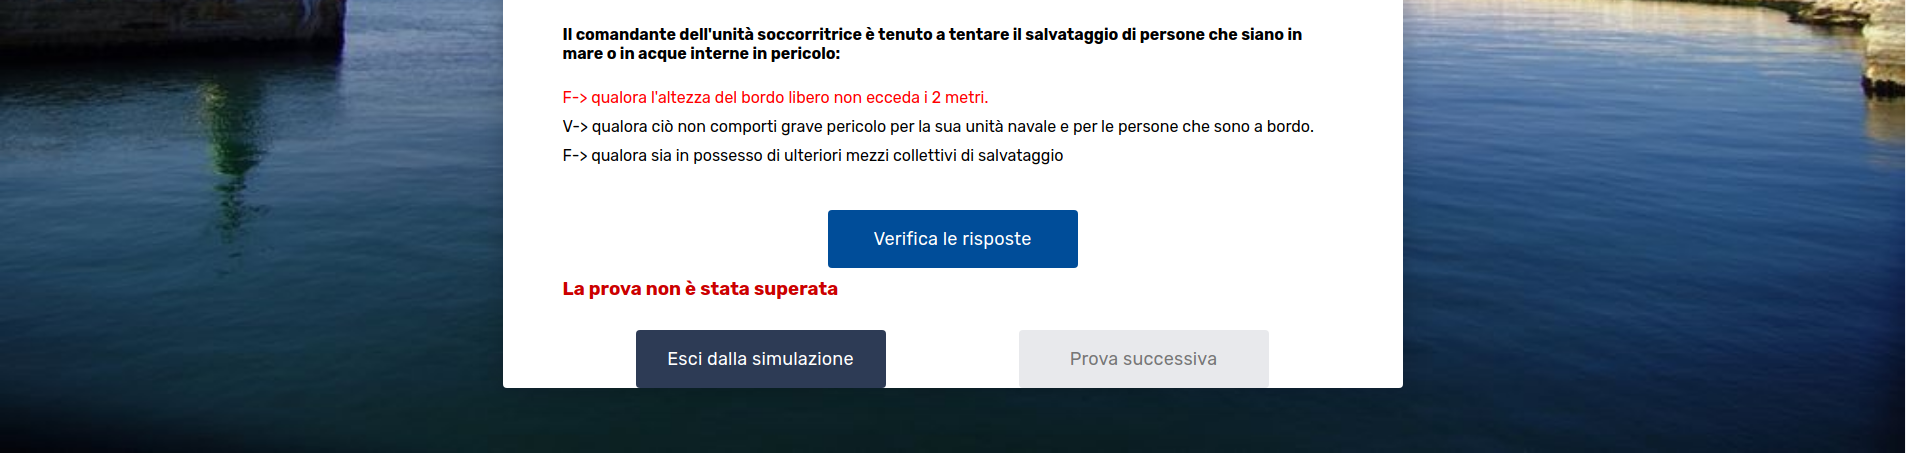
\includegraphics[scale=0.25]{Sites-images/37-Simulazione_quiz_base-risposte5.png}
		\caption{Pagina di simulazione dei quiz base con soluzioni.}
		(Ricomposta)
	\end{center}
\end{figure}

\textcolor{black}{Osservata la simulazione si analizza ora la parte di esercitazione associata alla simulazione.}\\

\paragraph{\textcolor{black}{Quiz base (esercitazione)}}\leavevmode\\
\textcolor{black}{L'unica novità rispetto al passato è il fatto che anche in questo esercizio si tiene il conto degli errori commessi. La problematica risiede sempre nella comunicazione tra "front-end" e "back-end", siccome è solo la parte del "javascript" che è in grado di verificare le risposte (la pagina mostra e corregge una domanda per volta). La soluzione (in linea con il passato) è stata quella di mettere in comunicazione questi due emisferi salvando dei parametri "nell'url", primo tra tutti il tipo di domande scelte come nel caso della esercitazione sulla prova di carteggio, date le problematica nel far funzionare "AJAX".\\
Qui di seguito è riportato il codice in "php".}\\

\begin{lstlisting}[language=php]
/*---------- CATCH URL VARIABLES ----------*/
$Array = $urlUtility->getInfoFromUrl($_SERVER['REQUEST_URI']);

//---------- CATCH SCORE
if($Array['score'] !== null){
	$_SESSION['score'] = $Array['score'];
}

//---------- CATCH LAST QUESTIONS VARIABLES
if($Array['index'] !== null && $Array['answer'] !== null){
	
	if($_SESSION['answeredQuestions'][$Array['index']] == null){
		$_SESSION['answeredQuestions'][$Array['index']] = $Array['answer']; 
	} 
}

//---------- CATCH TOPIC 
if($Array['topic'] !== null && $Array['topic'] !== $_SESSION['topic']){
	$_SESSION['topic'] = $Array['topic'];
	
	/*change temp array to determinate questions*/
	$query = $utilities->getMysql()->query("SELECT * FROM base_quiz WHERE (topic = '{$Array['topic']}')");
	$tempArray = $query->fetch_all(MYSQLI_ASSOC);
	/*format variables for question preparation part*/
	$_SESSION['maxQuestions']         = null;
	//get number of extracted questions
	$_SESSION['questions']            = $tempArray;
	$_SESSION['numbers']              = 0;
	$_SESSION['score']                = 0;
	$_SESSION['answeredQuestions']    = null;
}
\end{lstlisting}

\textcolor{black}{Nel codice appena mostrato vi è una funzionalità (implementata a livello di "php" con il "catch" dell'ultima risposta data, trasmessa dal "javascript") che permette di tenere in sessione le risposte date in precedenza in modo da poterle ricontrollare anche in un secondo momento. Il resto del codice in "php" non presenta differenze sostanziali rispetto a quanto è già stato mostrato  e anche il codice "html" è intuibile tenendo a mente quello scritto nel caso della simulazione.\\
Nel caso del "javascript" una cosa da evidenziare è l'inserimento dei parametri "nell'url" e anche come vengono gestire le riposte date in precedenza.}\\

\begin{lstlisting}[language=java]
	
	/*--------- SECTION WHERE VERIFY IF THE QUESTION WAS ANSWERED ----------*/
	//useful variables
	var questionIndex = <?php if($id !== null){echo $id;}else{echo "-1";}?>;
	var answerGiven = null;
	
	//verified the past answer
	if(Boolean(<?php if($_SESSION['answeredQuestions'][$id] !== null){echo true;}else{echo false;}?>)){
		
		// to not permit other review
		corrected = true;
		
		switch(<?php if($_SESSION['answeredQuestions'][$id] !== null) {echo $_SESSION['answeredQuestions'][$id];}else{echo "-1";} ?>){
			
			case <?php echo ANSWER1; ?>:
			
			answerRadios.style.display = "none";
			answer1.style.display      = "block";
			answer2_null.style.display = "block";
			answer3_null.style.display = "block";
			break;
			
			case <?php echo ANSWER2; ?>:
			
			answerRadios.style.display = "none";
			answer1_null.style.display = "block";
			answer2.style.display      = "block";
			answer3_null.style.display = "block";
			break;
			
			case <?php echo ANSWER3; ?>:
			
			answerRadios.style.display = "none";
			answer1_null.style.display = "block";
			answer2_null.style.display = "block";
			answer3.style.display      = "block";
			break;
			
		}
		
	}
	
	// set argument topic to url
	function setArgument(topic){
		var URL = window.location.href;
		var data ={'topic': topic};
		var parameters = new URLSearchParams(data);
		window.location.href = URL.split('?')[0]+"?"+parameters;
	}

	//set the new score to url
	function setScore(score){
		var URL = window.location.href;
		var data ={'score': score};
		var parameters = new URLSearchParams(data);
		window.history.pushState(null, document.title, (URL.split('?')[0]+"?"+parameters))
	}

	//set the answer given to php session by url
	function setAnswerGiven(index, answer){
		var URL = window.location.href;
	
		var data1 ={'index': index};
		var data2 ={'answer': answer};
		var parameters1 = new URLSearchParams(data1);
		var parameters2 = new URLSearchParams(data2);
		window.history.pushState(null, document.title, (URL+"&"+parameters1+"&"+parameters2));
	}
\end{lstlisting}\leavevmode\\
\textcolor{black}{Purtroppo anche in questa situazione non potendo utilizzare "AJAX" si sono dovuti trovare dei "workaround" per permettere comunque l'implementazione di queste funzionalità ritenute importanti.\\
Nel caso in cui nella pagina venga caricata una domanda alla quale si è già risposto, viene eseguita in automatico la correzione, prendendo come valore per la risposta data in precedenza.\\
Altra cosa qui mostrata è come sono stati salvati tutti i paramatri "nell'url" in modo da poter essere poi ripresi dalla parte in "php".}\\

\begin{figure}[h]
	\begin{center}
		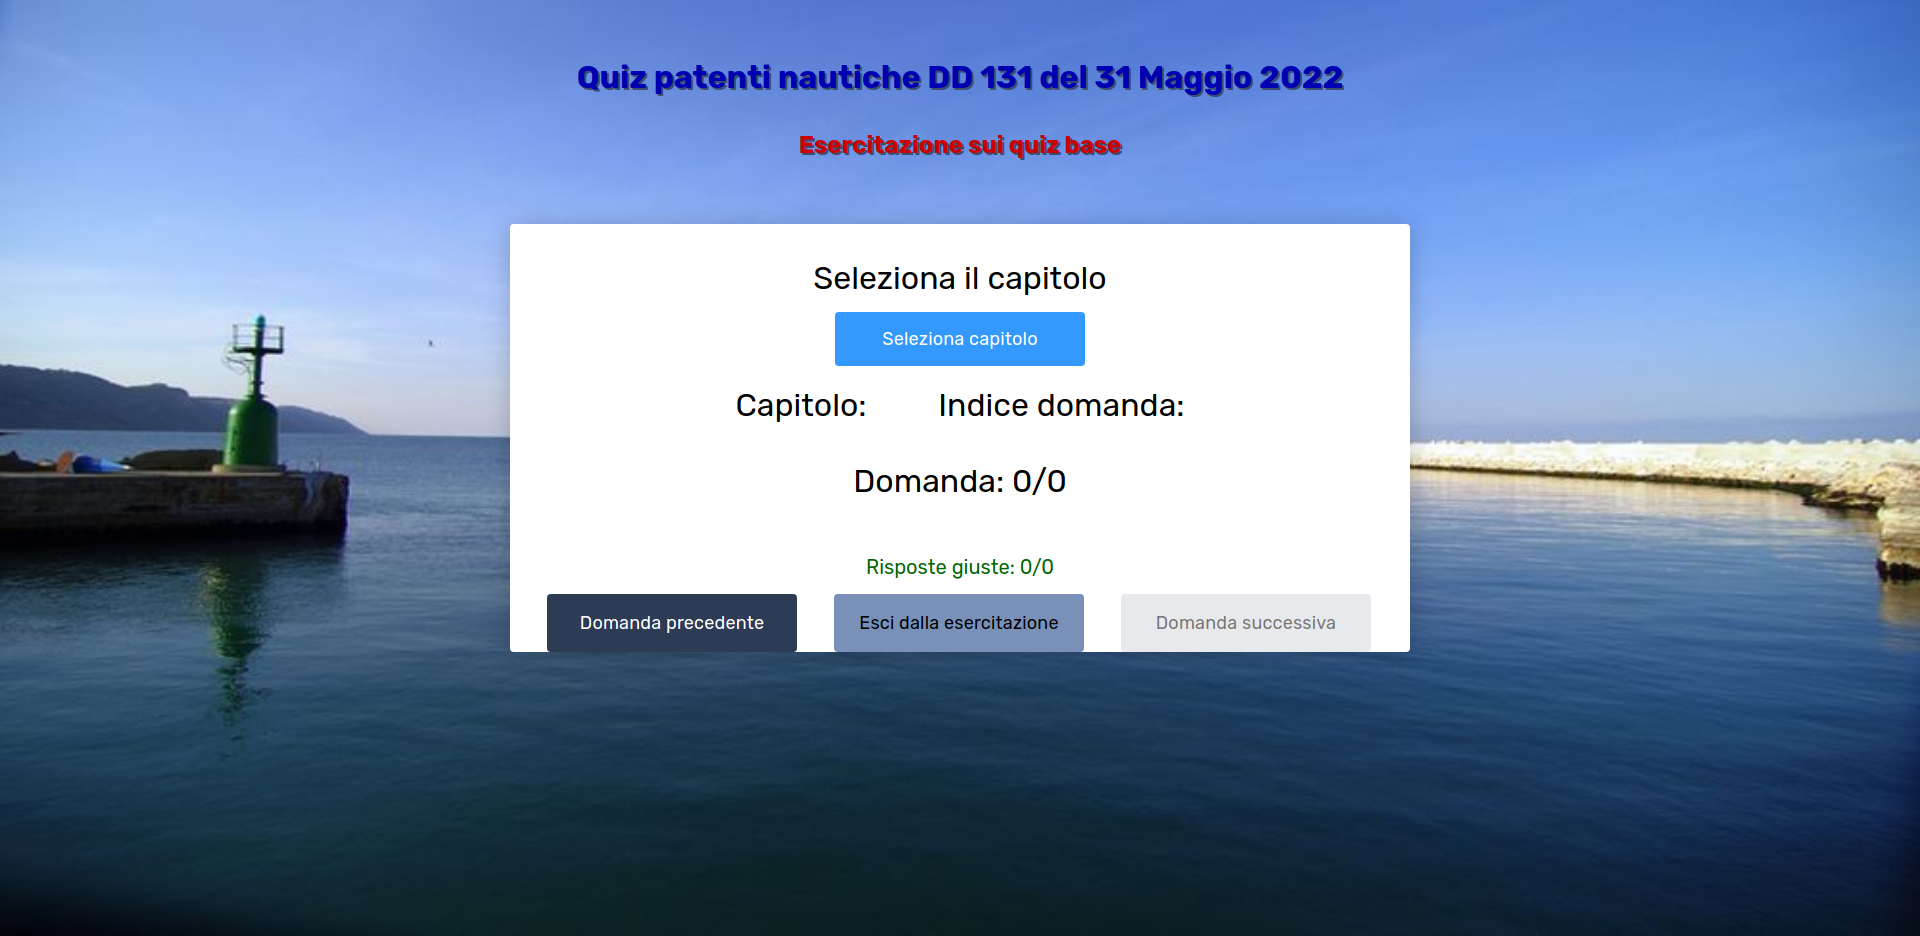
\includegraphics[scale=0.25]{Sites-images/38-Quiz_Base.png}
		\caption{Pagina dei quiz base.}
	\end{center}
\end{figure}

\begin{figure}[h]
	\begin{center}
		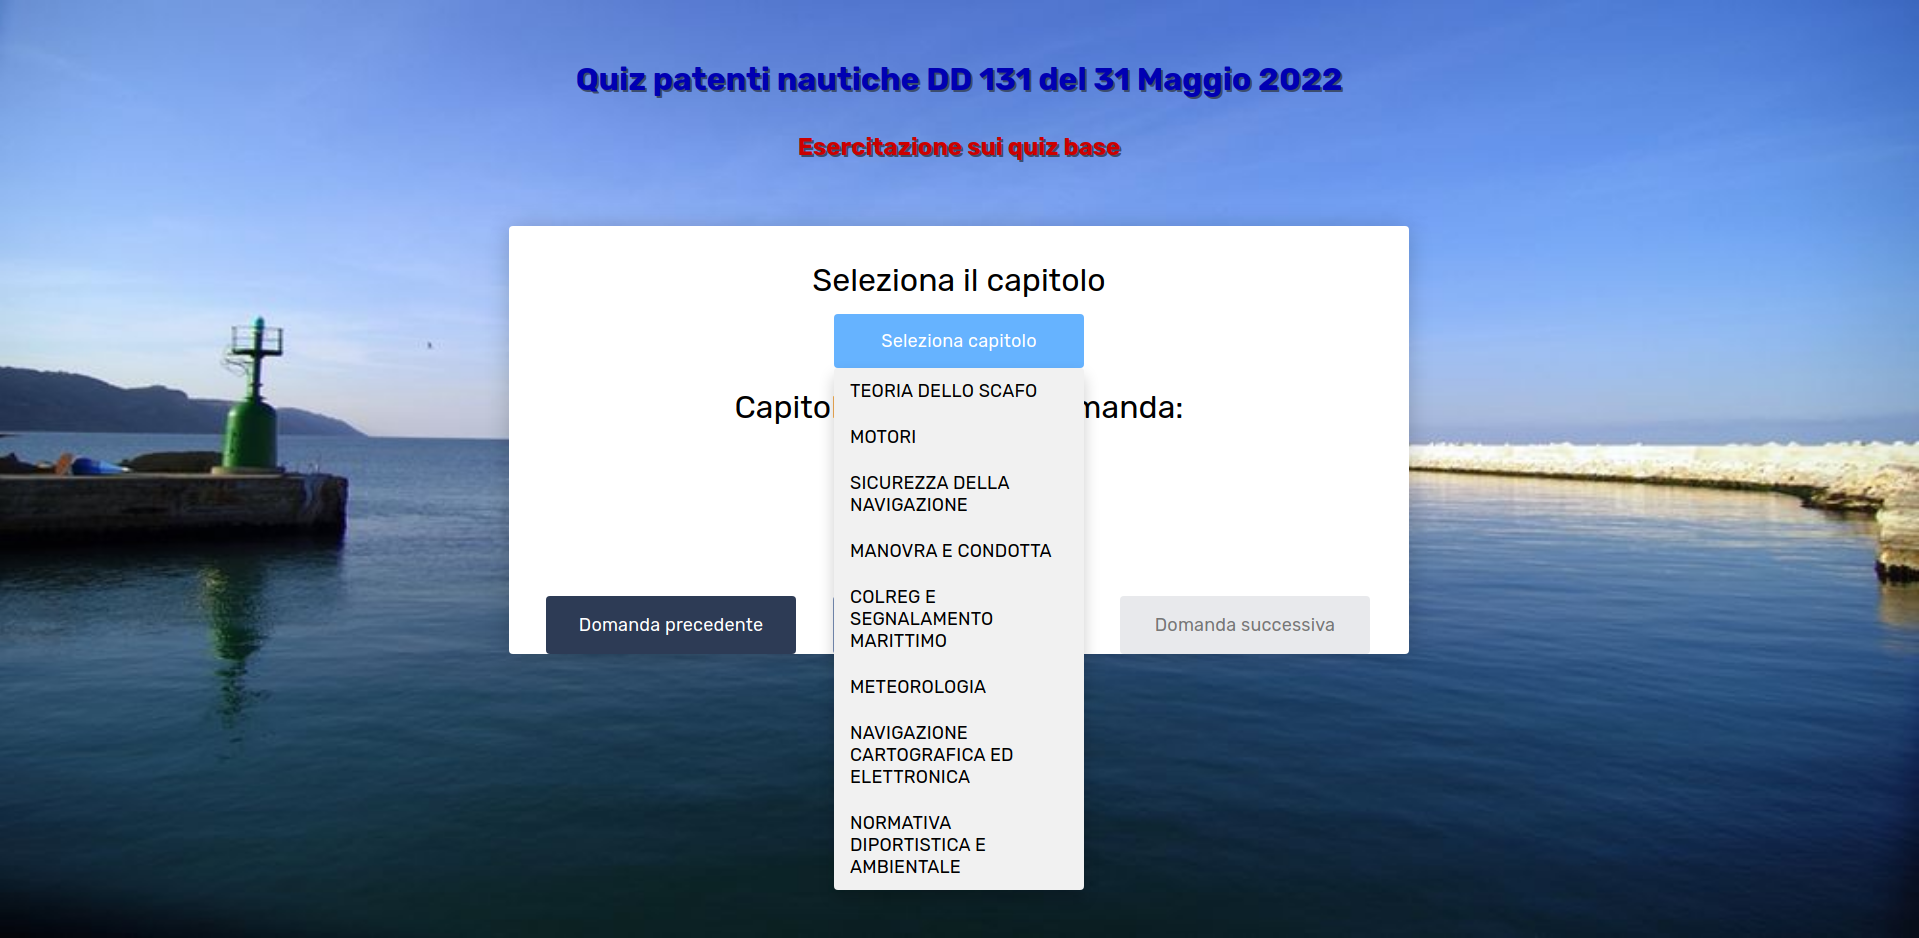
\includegraphics[scale=0.25]{Sites-images/39-Quiz_Base_selezione.png}
		\caption{Pagina dei quiz base con selezione.}
	\end{center}
\end{figure}

\begin{figure}[h]
	\begin{center}
		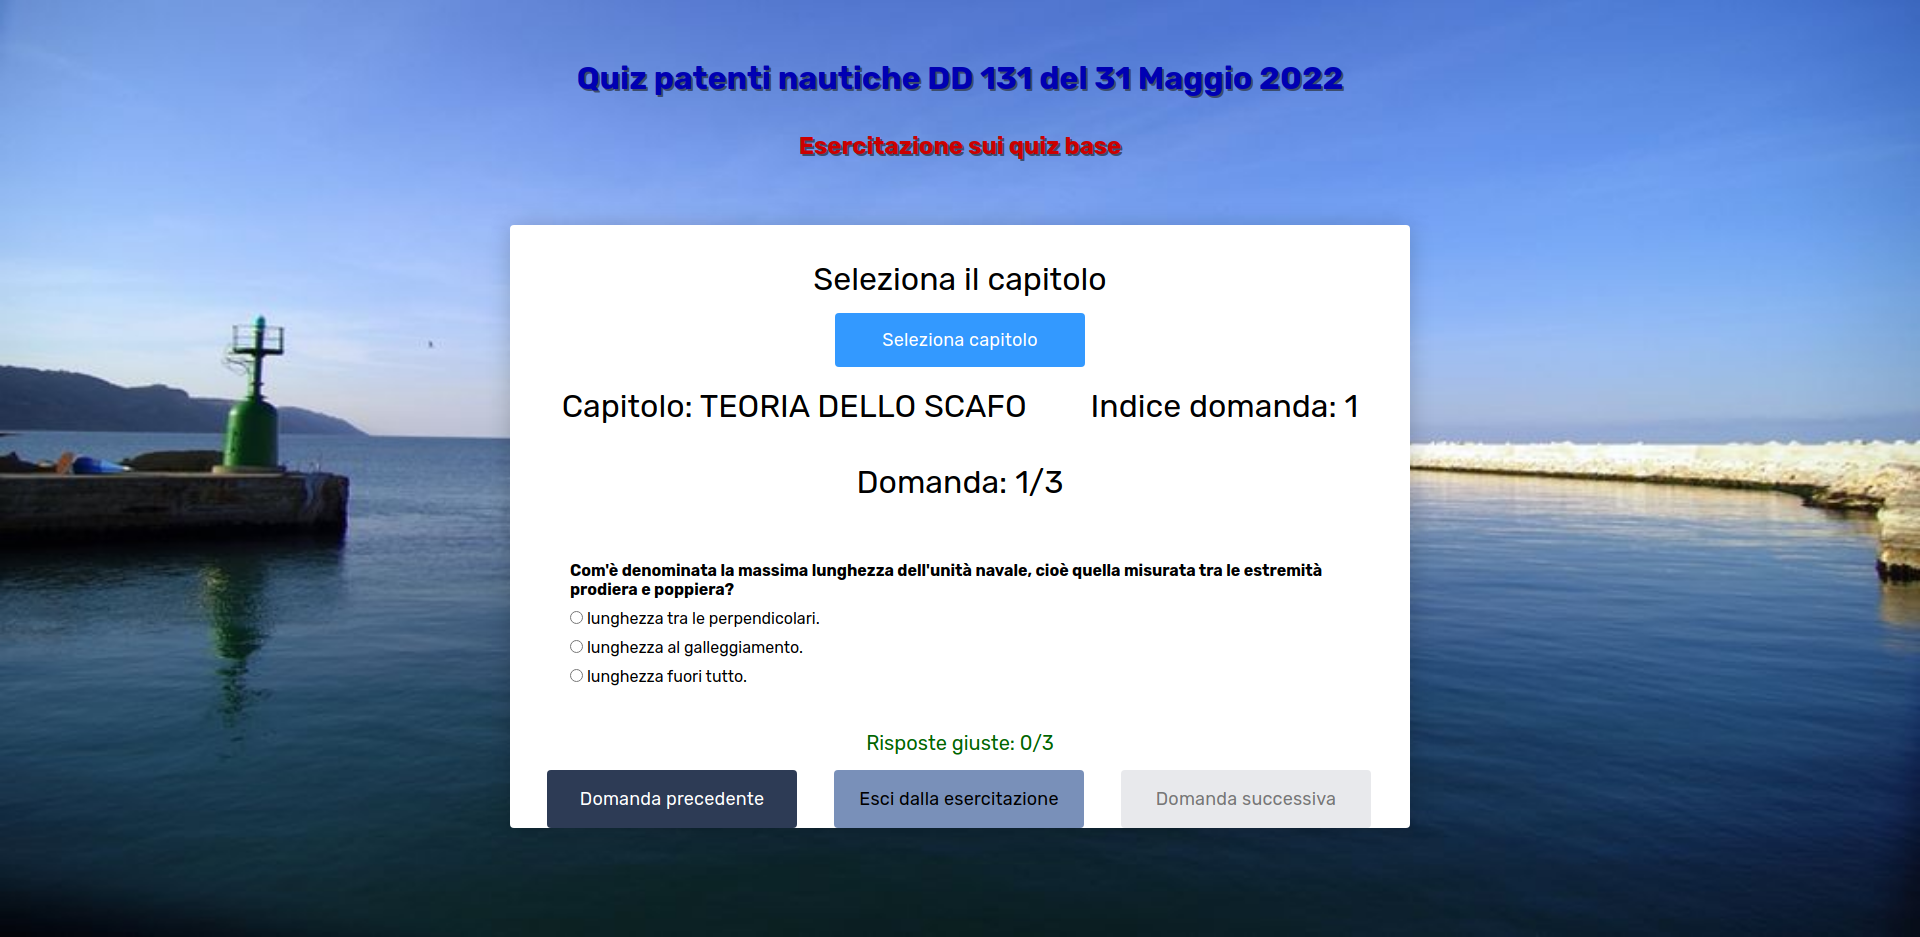
\includegraphics[scale=0.25]{Sites-images/40-Quiz_Base_Domanda.png}
		\caption{Pagina dei quiz base con domanda.}
	\end{center}
\end{figure}

\begin{figure}[h]
	\begin{center}
		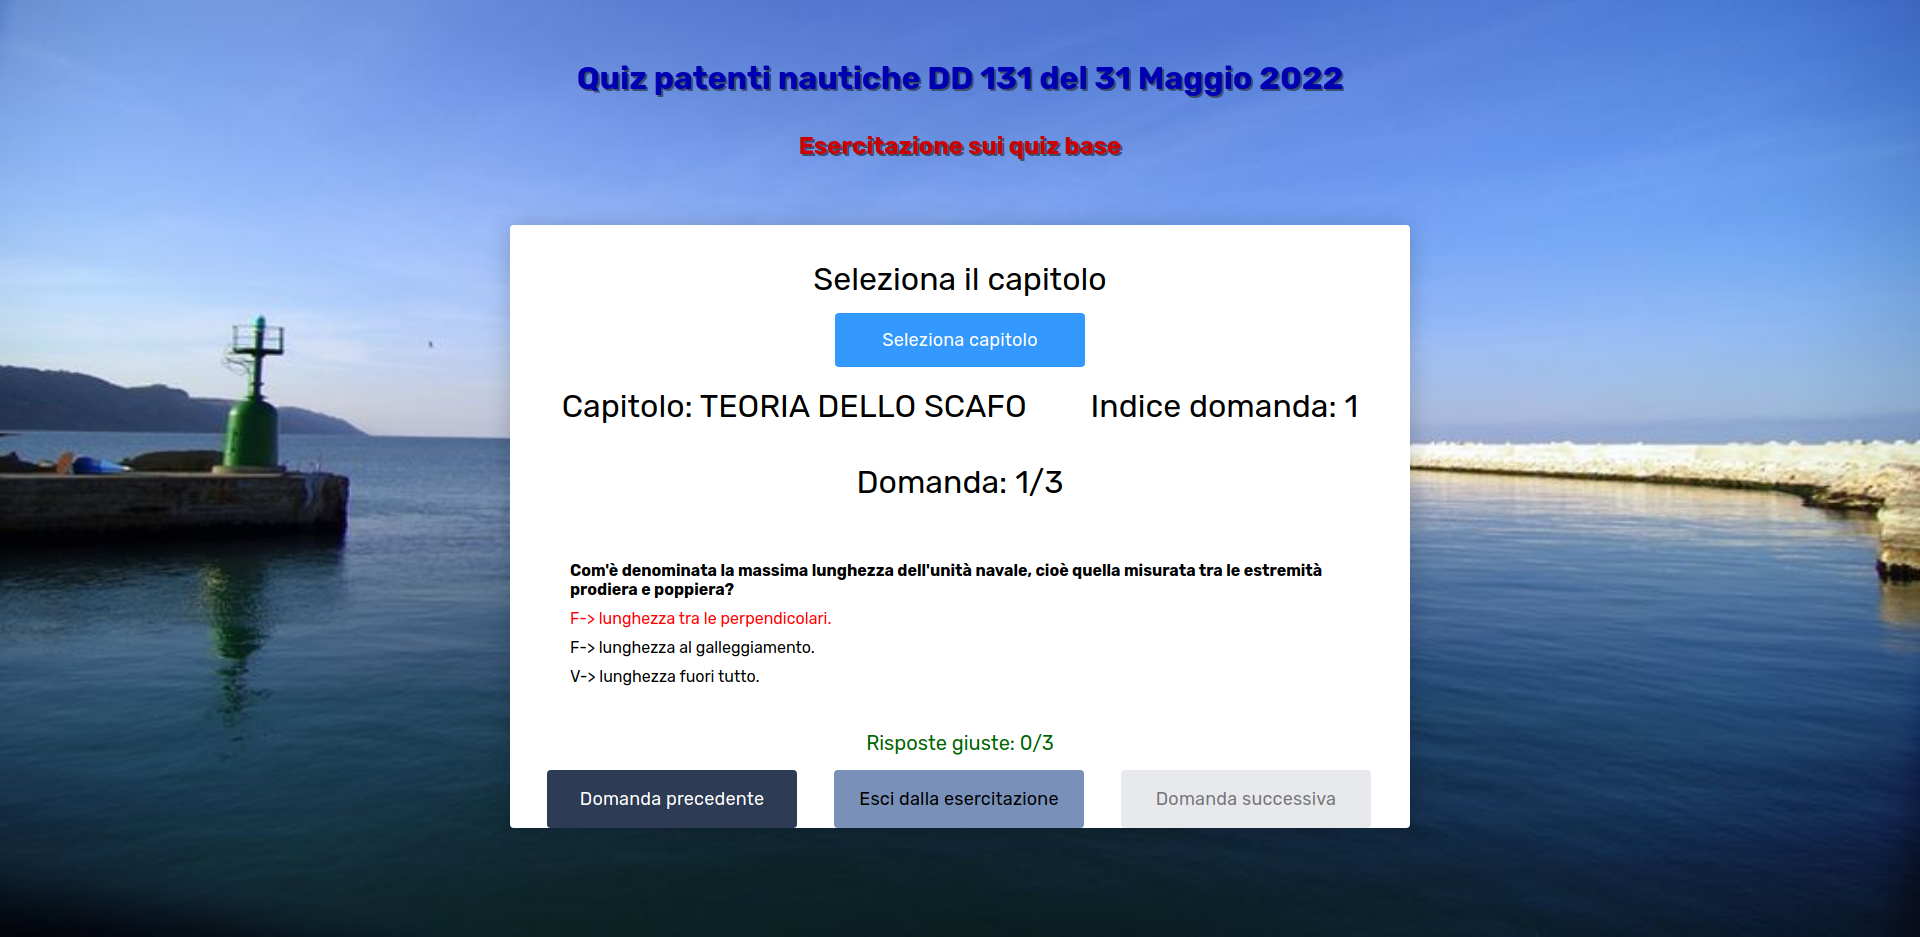
\includegraphics[scale=0.25]{Sites-images/41-Quiz_Base_Soluzione.png}
		\caption{Pagina dei quiz base con soluzione.}
	\end{center}
\end{figure}

\textcolor{black}{L'ultima parte del sito implementata, ovvero la simulazione e l'esercitazione dei quiz della vela non viene riportata, in quanto sulla base di quello che è stato mostrato finora sarebbe irrilevante, poiché ripetizione di logiche e di codice già visto.} 